% Template para Proposta e TCC da EST/UEA -
% Padrão para os cursos do Núcleo de Computação
%
% Elaborado por Elloá B. Guedes
% Adaptado da versão elaborada por:				%                   Jucimar Maia Jr.
%
% Versão beta - 08 de outubro de 2015
%
\documentclass[a4paper,titlepage,12pt]{report}


\usepackage[utf8]{inputenc}
\usepackage[OT1]{fontenc}
\usepackage{ae}
\usepackage[brazil]{babel}
\usepackage{a4wide}
\usepackage{comment}
\usepackage[pdftex]{graphicx,color}
\usepackage{graphics}
\usepackage{cite}
\usepackage{longtable}
\usepackage{float}
\usepackage{fancyvrb}
\usepackage{fancyhdr}
\usepackage{setspace}
\usepackage{amsmath}
\usepackage{lscape}
\usepackage{textcase}
\usepackage{anysize}
\usepackage{setspace}
\usepackage{booktabs}
\usepackage{url}
\usepackage{subfig}
\usepackage{cite}
\usepackage[alf]{abntex2cite}

\marginsize{20mm}{20mm}{20mm}{15mm}


%% Cabeçalhos
\renewcommand{\topfraction}{1}
\renewcommand{\bottomfraction}{1}
\renewcommand{\floatpagefraction}{1}
\renewcommand{\textfraction}{0}
%\renewcommand{\baselinestretch}{2}
\doublespacing %espaçamento duplo
\sloppy

%% Nomes
\floatstyle{plain}  %%% tipos: plain, boxed, ruled
\newfloat{codigo}{tbp}{lop}[section]
\floatname{codigo}{Código}

%%% nome para ser usado no sumário

\newcommand{\listofcodename}{Lista de C\'{o}digos}



% RESUMO ----------------------------------------------------------------------------------------------------------------------------------------------------------------------

\newcommand{\resumo}[1]{
\begin{center} \LARGE \bf Resumo \end{center}

\vskip 4em
\input{#1}

\newpage

}

% ABSTRACT ----------------------------------------------------------------------------------------------------------------------------------------------------------------------

\newcommand{\abstractt}[1]{
\begin{center} \LARGE \bf Abstract \end{center}

\vskip 4em
\input{#1}

\newpage

}

% Sumário -----------
\newcommand{\sumario}{
\renewcommand{\contentsname}{Sum\'{a}rio}
\tableofcontents
% \addcontentsline{toc}{chapter}{\listtablename}
% \listoftables

\newpage
\addcontentsline{toc}{chapter}{\listfigurename}
\listoffigures
% \addcontentsline{toc}{chapter}{\listofcodename}
% \listof{codigo}{\listofcodename}  % Lista de Códigos

\clearpage
}

\pagestyle{plain}

\newcommand{\folhaRosto}[6]{

\thispagestyle{empty}
\begin{center}
\textbf{\\[0.4em]\MakeUppercase{#2} \\[5cm]}
\textbf{\MakeUppercase{#1}\\[96pt]}

\end{center}

\hspace*{8cm}
\begin{minipage}{8cm}
Trabalho de Conclus\~{a}o de Curso
apresentado \`{a} banca avaliadora do Curso de Sistema de Informa\c{c}\~{a}o, da
Escola Superior de Tecnologia, da Universidade do Estado do Amazonas, como
pr\'e-requisito para obten\c{c}\~{a}o do t\'{\i}tulo de bacharel.\\[40pt]
\end{minipage}

\begin{center}
Orientador(a): #3 \\
Coorientador(a): #6\\[12ex]
Manaus -- #4 -- #5\\
\end{center}


\pagenumbering{roman}
\newpage
}




%% Preencha aqui os seguintes dados
\def \titulo{Sistema de auditoria baseado em Blockchain para o aplicativo do Restaurante Universitário da UEA}
\def \orientador{Profa. MSc. Cristina Souza de Araújo}
\def \coorientador{Prof. Dr. Jucimar M. da Silva Junior}

\def \nome{Luiz Carlos Glomyer Pereira Gomes Junior}
\def \mes{Março}
\def \ano{2023}

\begin{document}

\folhaRosto{\titulo}{\nome}{\orientador}{\mes}{\ano}{\coorientador}

% Edite os seguintes arquivos para alterar as informações necessárias
% ficha Catalográfica------------------------------------------------------------------------------------------------------------------------------------------
\begin{spacing}{1.4}
\textit{\textbf{\\
Universidade do Estado do Amazonas - UEA\\
Escola Superior de Tecnologia - EST}}

\textit{\\
Reitor:\\
\textbf{André Luiz Nunes Zogahib}\\
Vice-Reitor:\\
\textbf{Kátia do Nascimento Couceiro}}
\\
\textit{
Diretor da Escola Superior de Tecnologia:\\
\textbf{Ingrid Sammyne Gadelha Figueiredo}}
\\
\textit{
Coordenador do Curso de Sistemas de Informação:\\
\textbf{Marcela Sávia Picanço Pessoa}}
\\
\textit{
Coordenadora da Disciplina Projeto Final:\\
\textbf{Polianny Almeida Lima}}
\\[12pt]
\textit{
Banca Avaliadora composta por: \hfill Data da Defesa: 28/03/2023.\\
}
\textit{
\textbf{Profa.  MSc. Cristina Souza de Araújo} (Orientadora)\\
\textbf{Prof. Dr. Luis Cuevas Rodriguez}\\% Escreva o nome dos professor da sua banca antes de '\\' (comando para quebra de linha)
\textbf{Prof. MSc. Eduardo Jorge Lira Antunes da Silva}
}
\center{\bf CIP -- Catalogação na Publicação}\ \ \\
 \begin{small}
\begin{center}
\fbox{
\parbox{18cm}{
\begin{minipage}{17cm}
L864a \hspace*{1cm} Junior, Luiz Carlos Glomyer Pereira Gomes\\[12pt]
\hspace*{2cm} \parbox{14cm}{
\hspace*{0.5cm}Sistema de auditoria baseado em Blockchain para o aplicativo do Restaurante Universitário da UEA [orientado por] Profa. MSc. Cristina Souza de Araújo -- Manaus: UEA, 2023.\\
\hspace*{0.5cm}240 p.: il.; 30cm\\
\hspace*{0.5cm}Inclui Bibliografia\\
\hspace*{0.5cm}Trabalho de Conclus\~{a}o de Curso (Gradua\c{c}\~{a}o em Sistemas de Informação).
Universidade do Estado do Amazonas, 2023.\\[6pt]
\hspace*{8cm} CDU: \hrulefill}
\end{minipage}}}
\end{center}
\end{small}
\end{spacing}
 \newpage

% folha de aprovação----------------------------------------------------------------------------------------------------------------------------------

\begin{center}
\bf \MakeUppercase{\nome}\\[1.5 cm]
\end{center}

\begin{center}
\bf \MakeUppercase{\titulo}\\[1.5cm]
\end{center}

\hspace*{8cm}
\begin{minipage}{8cm}

Trabalho de Conclus\~{a}o de Curso apresentado \`{a}
banca avaliadora do Curso de Sistemas de Informação,
da Escola Superior de Tecnologia, da Universidade do Estado do Amazonas,
como pr\'e-requisito para obten\c{c}\~{a}o do t\'{\i}tulo de bacharel.\\

\large \bf Aprovado em: 28/03/2023
\end{minipage}

BANCA EXAMINADORA\\[12 pt]

\noindent \hrulefill \hspace*{6cm} \\
\noindent \textbf{\orientador}\\
\textit{UNIVERSIDADE DO ESTADO DO AMAZONAS}\\[0.5cm]

\noindent \hrulefill \hspace*{6cm} \\
\noindent \textbf{Prof. Dr. Luis Cuevas Rodriguez}\\
\textit{UNIVERSIDADE DO ESTADO DO AMAZONAS}\\[0.5cm]

\noindent \hrulefill \hspace*{6cm} \\
\noindent \textbf{Prof. Msc. Eduardo Jorge Lira Antunes da Silva}\\
\textit{UNIVERSIDADE DO ESTADO DO AMAZONAS}\\



% Indique onde esta o arquivo do resumo
\resumo{./files/resumo.tex}
% Idem para o abstract
\abstractt{./files/abstract.tex}
 
\begin{center} \LARGE \bf Agradecimentos \end{center}

\vskip 4em
Agradeço primeiramente à Deus pelo dom da vida e da existência.

Agradeço aos meus pais por todo o seu suporte e empenho, principalmente durante o período dificultoso que foram estes últimos semestres da universidade. Sem eles eu não chegaria onde cheguei e nem seria pessoa que sou hoje.

Agradeço aos meus orientadores. À professora Cristina pelos excelentes direcionamentos e \emph{feedbacks} dados, principalmente quanto ao trabalho escrito e apresentação. Ao professor Jucimar pelas orientações e por ceder o espaço e os materiais necessários para o desenvolvimento deste trabalho.

Agradeço aos meus amigos e companheiros de universidade, sem eles a jornada pela vida universitária não seria nada fácil.

Agradeço à professora Marcela, coordenadora do curso de Sistemas de Informação, que está sempre disposta a ajudar e resolver os problemas dos alunos do curso.

Agradeço ao Lucas Lima, desenvolvedor do \emph{back-end} do aplicativo do RU, que me auxiliou com os aspectos-chave do sistema que tive contato.

Agradeço à UEA, por oferecer ensino de qualidade de maneira democrática e aberta e pelas diversas oportunidades aos alunos, sobretudo do núcleo de computação.

À Diane.

\newpage





\sumario

% Configuração de cabeçalhos
\pagestyle{fancy}
\renewcommand{\chaptermark}[1]{\markboth{#1}{}}
\renewcommand{\sectionmark}[1]{\markright{#1}}
\renewcommand{\headrulewidth}{0.5pt}
\newcommand{\rom}{\fontfamily{cmr}\fontseries{m}\fontsize{10}{12}\selectfont}
\fancyhf{} \fancyhead[LE,RO]{\rom\thepage}
\fancyhead[LO]{\rom\rightmark} \fancyhead[RE]{\rom\leftmark}
\fancypagestyle{plain}{
    \fancyhead{} % get rid of headers
    \renewcommand{\headrulewidth}{0pt} % and the line
 }


\pagenumbering{arabic}



% Seus capítulos vão aqui --------
\chapter{Introdução}


%-----------------------------------------
%-----------------------------------------
\section{Descrição do Problema}

Em um mundo altamente globalizado e de tecnologias emergentes, empresas se veem na necessidade de modernizarem a si mesmas em face à grande competitividade existente. Grandes, médios, pequenos e micro negócios tiveram de se adequar às demandas dessa nova realidade, sobretudo no que diz a respeito da informatização de processos, com o intuito de lograr rapidez e eficiência. Daí surge a chamada agilidade operacional, a tendência de tornar estes processos dinâmicos e flexíveis.

A Universidade do Estado do Amazonas (UEA) é a maior universidade multicampi do país, sendo composta por vinte e três unidades diferentes, possuindo mais de vinte mil alunos matriculados em sua totalidade. Apesar de ser uma instituição de ensino de grande porte, vários de seus processos internos estão de certa forma defasados, demandando mais recursos humanos que o necessário, consequentemente acarretando em perdas operacionais, e até mesmo monetárias. 

O RU (Restaurante Universitário) é o local encarregado de prover aos alunos, técnicos e professores da instituição refeições diversificadas e de qualidade por um preço acessível ao público, contemplando uma refeição para cada turno do dia: café da manhã pelo turno da manhã, almoço pelo turno da tarde e lanche pelo turno da noite. Para fazer uso do Restaurante Universitário, o aluno deve, primeiramente, emitir uma carteirinha própria da UEA.

Apesar de cumprir o seu objetivo primário, o RU é uma área da universidade tida por grande parte dos alunos como insatisfatória, sobretudo no que vem a ser o seu fluxo de atendimento: o aluno, munido de sua carteirinha de estudante, deve enfrentar longas filas para realizar a compra de um ticket de alimentação, para então novamente enfrentar outra fila, desta vez para obter de fato a sua refeição.

Com isso, perdas notáveis ocorrem no convívio diário dos alunos dentro da universidade. Visto que muitos não conseguem se alimentar em tempo hábil, os discentes que optam por não almoçar vão à sala de aula com fome, minando assim o desempenho que outrora possuiriam caso estivessem bem alimentados. Outra parte dos usuários do local dedica um esforço a obter comida de outras fontes, uma alternativa que acaba sendo monetariamente cara, se comparada ao preço convidativo do Restaurante Universitário, ou até mesmo maléfica para a saúde, caso o aluno opte por comer fast-food ou comidas pré-prontas.

Além dos alunos, parte do corpo docente e dos técnicos gerais da universidade também frequenta o restaurante, agravando ainda mais a situação já precária. Felizmente, uma solução para esta problemática está em andamento, que é o desenvolvimento de uma aplicativo para dispositivos móveis para dar suporte ao RU.

No entanto, surge um desafio na implementação desta solução: garantir segurança nas informações armazenadas. Segundo dados de um estudo da Roland Berger, empresa alemã de consultoria estratégica, em 2021 o Brasil foi o 5° maior país a sofrer ataques cibernéticos \cite{SecurityReport}, sobretudo ataques de ransomware, modalidade de ataque que consiste em tornar as vítimas reféns ao demandar o pagamento de um resgate para recobrar o acesso aos seus próprios dados.  O ranking National Cyber Security Index \cite{NCSI}, um índice global que mede o preparo e a prontidão dos países para lidar com ciberataques, figura o Brasil na 68° com um índice de cibersegurança de 51.95 (Figura \ref{fig:ncsi}); em comparação com a Grécia, que ocupa o primeiro lugar com ranking de 96.10, observamos uma enorme disparidade.

\begin{figure}
    \centering
    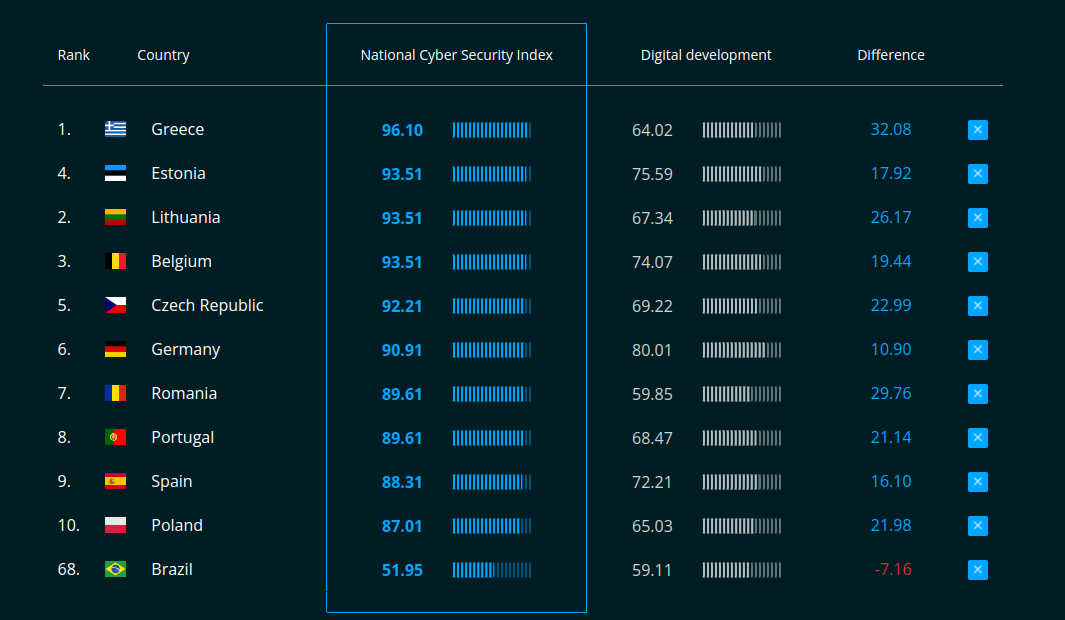
\includegraphics[width=1\textwidth]{img/Cap1/NCSI ranking.png}
    \caption{Ranking NCSI de cibersegurança global \cite{NCSI}}
    \label{fig:ncsi}
\end{figure}

Casos como o ataque de ransomware sofrido pelas lojas Renner \cite{TheHack} nos reforçam a importância de investir em segurança ao se desenvolver um software. As consequências de um ataque deste tipo não são apenas financeiras, mas também operacionais, resultando em indisponibilidade em sistemas de informação. A depender da aplicação, esta indisponibilidade pode ser fatal, afetando vidas humanas. Um dos maiores casos de ciberataque da história afetou diversos hospitais de um serviço de saúde dos Estados Unidos, minando os atendimentos e visualização de dados de pacientes, obrigando os colaboradores a recorrerem ao uso de papel e caneta \cite{NBCNews}. E este cenário tende a piorar: análises de \cite{CheckPointResearch} indicam que a taxa de ciberataques globais sofreu um aumento de 42\% no ano de 2022.
 
Incidentes em que há perda de posse de informações privadas, casos de roubo ou adulteração de dados sensíveis (que muitas vezes passam despercebidos pois são de difícil identificação) e episódios de indisponibilidade de dados podem ser evitados pelo uso da tecnologia Blockchain. A Blockchain possibilita contornar esses e outros problemas de segurança capazes de acometer um sistema computacional devido às suas particularidades. Considerada por diversos especialistas como uma tecnologia revolucionária e disruptiva devido ao seu enorme potencial \cite{Ejeke2022}, é uma das precursoras da chamada Web 3.0, uma evolução da rede mundial de computadores com foco na descentralização da informação.

A Blockchain é uma tecnologia que consiste em um conjunto de registros, os blocos, que são encadeados por meio de criptografia. Funciona como uma espécie de livro-razão: operações efetuadas na rede, as chamadas transações, são registradas e validadas de tempos em tempos. Após aproximadamente dez minutos essas transações são coletadas e agregadas em um único bloco, que por sua vez passa então por um processo de validação, sendo finalmente anexado no final da Blockchain, formando uma ligação com o último bloco armazenado anteriormente armazenado. Esse processo de validação de bloco se chama mineração e é necessário para garantir que os dados lá armazenados sejam íntegros e fidedignos à realidade. Usando a Blockchain como um repositório de dados conseguimos implementar um sistema seguro e à prova de ataques.


% \newpage %%
%-----------------------------------------
%-----------------------------------------
\section{Objetivos}

\subsection{Objetivo Geral}

O objetivo deste trabalho é desenvolver um sistema de registros (\emph{logs}) baseado na tecnologia Blockchain para o aplicativo Carteira Digital do Restaurante Universitário da UEA, fornecendo assim suporte à auditorias e análises do funcionamento do sistema em face à utilização por parte do usuário.

\subsection{Objetivo Específico}
O objetivo geral pode ser decomposto nos seguintes itens:
\begin{enumerate}
    \item Desenvolver um sistema de suporte a processos de auditoria por meio de uma API para o aplicativo Carteira Digital do Restaurante Universitário da UEA;
    \item Implementar comunicação com a Blockchain Ethereum e utilizá-la para garantir segurança à aplicação;
    \item Criar \emph{endpoints} na aplicação para tornar possível registro e leitura de informações de uso do sistema;
    \item Realizar integração entre o sistema desenvolvido e o \emph{back-end} do aplicativo Carteira Digital do Restaurante Universitário da UEA;
    \item Tornar possível a realização de auditorias no sistema.
\end{enumerate}


%-----------------------------------------
%-----------------------------------------
\section{Justificativa}
Visto os problemas enfrentados por quem frequenta o Restaurante Universitário, o desenvolvimento de uma aplicação é uma proposta de solução eficaz para sanar as irregularidades presenciadas no processo de atendimento do restaurante.

Esta solução, uma vez implementada, testada e implantada, tem o potencial de contemplar as demais unidades da Universidade do Estado do Amazonas. No entanto, sua utilização de modo massivo abre brechas à incidentes de segurança.

Registrar as ações tomadas pelos usuários no sistema nos garante retratabilidade, permitindo assim a identificação de entidades maléficas ou prejudiciais ao sistema. No entanto, surge um desafio quanto à privacidade do usuário, visto que todo o seu histórico poderia estar exposto em um eventual vazamento de dados, ou até mesmo sofrer adulteração por parte dos administradores do sistema. Vem à tona neste contexto a Blockchain, tecnologia capaz de garantir aspectos-chave quanto à privacidade do usuário.

\cite{Tapscott2016} afirma que medidas de segurança estão incorporadas na rede sem nenhum ponto de falha; qualquer usuário que utilizar de maneira maléfica os recursos da rede será, inevitavelmente, punido, garantindo assim uma rede segura e livre de agentes maliciosos.

%-----------------------------------------
%-----------------------------------------
\section{Metodologia}

A metodologia de desenvolvimento de \emph{software} utilizada para a elaboração deste projeto foi o modelo em cascata. Nela, o desenvolvimento da aplicação segue um caminho retilíneo: a análise de requisitos leva à estruturação do projeto, que por sua vez leva à implementação e posteriormente a entrega do projeto, com o último passo sendo a manutenção \cite{Pressman2021-jj}. Como o escopo da aplicação é bem definido, o modelo em cascata se prova como a abordagem mais eficiente para este cenário, diminuindo assim os riscos envolvidos com o processo de desenvolvimento.

Para gerenciar o código-fonte produzido, foram utilizadas as tecnologias Git e GitHub. O Git é um sistema de controle de versão originalmente desenvolvido por Linus Torvalds em 2005.  Um sistema de controle de versão gerencia diferentes versões de objetos criado durante a etapa de desenvolvimento a partir de procedimentos e ferramentas próprios \cite{Pressman2021-jj}. Com ele é possível ter um controle sobre as mudanças que ocorrem em um projeto, sobretudo dos artefatos produzidos durante o processo de desenvolvimento. A plataforma GitHub, por sua vez, fica encarregada de hospedar os artefatos de forma remota, em um servidor online, agindo tanto como uma cópia de segurança quanto uma maneira de divulgação e acesso do projeto. Além disso, optou-se por utilizar a língua inglesa no desenvolvimento da aplicação para tornar o projeto mais homogêneo e aumentar o seu possível alcance.

Para o desenvolvimento do software em si, foram definidas duas linguagens de programação principais: Python e Solidity. Uma API criada em Flask é o intermediário entre sistema e Blockchain, ficando encarregado de concretizar a comunicação entre ambas as partes. Para isso, a linguagem de programação Python foi escolhida por diversos motivos: 
\begin{itemize}
    \item Simplicidade em sua sintaxe, fornecendo maior legibilidade e entendimento do código;
    \item Grande suporte, devido a sua extensa comunidade de desenvolvedores e bibliotecas disponíveis;
    \item Alta portabilidade, tornando possível a migração do sistema para diversos outros sistemas operacionais.
\end{itemize}

Solidity, por sua vez, é uma das principais linguagens para implementação de contratos inteligentes em uso. Extensamente documentada, é a linguagem mais popular e a mais frequentemente utilizada para o desenvolvimento de contratos inteligentes na plataforma Ethereum \cite{Antonopoulos2018-jt}. Possui uma sintaxe similar a outras linguagens de programação, como C++ e Javascript. O contrato inteligente fica encarregado de salvar e recuperar os dados de tentativas de acesso na Blockchain.

Para realizar a comunicação entre aplicação e Blockchain, é utilizada a plataforma Infura, fornecendo uma interface que garante acesso instantâneo na plataforma Ethereum via HTTPS ou WebSockets, resultando em acessos mais rápidos e mais agilidade no processo de desenvolvimento, já que por meio do uso desta plataforma não é necessário destinar esforços para executar uma instância da plataforma Ethereum de forma local. Para compilar e implantar contratos inteligentes na Blockchain, o ambiente de desenvolvimento integrado Remix IDE (Figura \ref{fig:remix}) foi utilizado, junto com a extensão MetaMask. MetaMask é uma extensão de navegador que permite a comunicação entre dispositivos que não suportam o padrão de aplicações descentralizadas com uma rede Blockchain, permitindo executar operações na rede, além de também gerenciar carteiras virtuais utilizadas.

\begin{figure}
    \centering
    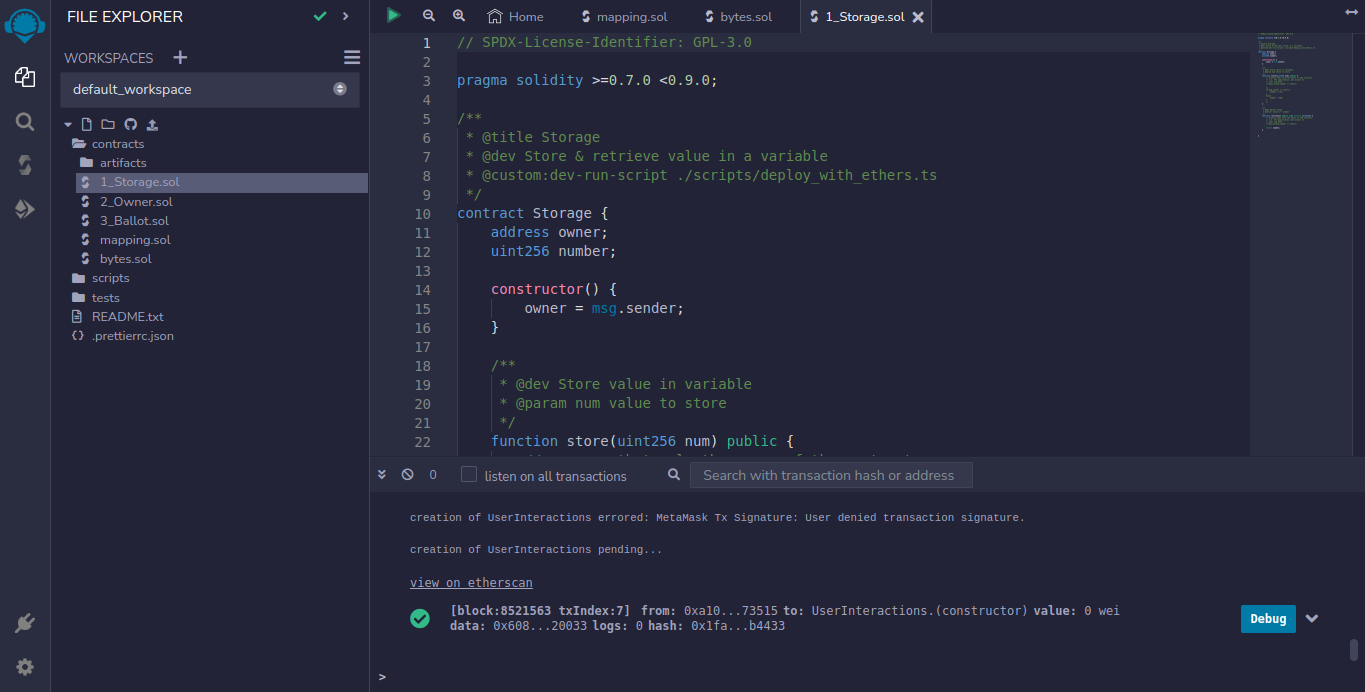
\includegraphics[width=1\textwidth]{img/Cap1/remix ide.png}
    \caption{Ambiente de Desenvolvimento Integrado Remix}
    \label{fig:remix}
\end{figure}

\chapter{Fundamentação Teórica}



\section{Linguagem de programação}
Uma linguagem de programação é uma linguagem artificial usada para controlar o comportamento de uma máquina. Aquele que manipula a máquina por meio de linguagens de programação é chamado de programador. Na prática, programadores utilizam linguagens de programação a fim de solucionar problemas de um determinado domínio. Há uma vasta gama de linguagens disponíveis a serem utilizadas, portanto os programadores devem possuir a capacidade de analisar e entender o problema tratado a fim de se escolher a linguagem mais adequada à situação \cite{Sebesta2011}. 

As linguagens costumam ser separadas em relação ao seu grau de abstração, quanto maior for a abstração, mais o programa escrito será intuitivo e se assemelha-rá com a linguagem falada; entretanto, maiores também serão os detalhes que se tornam inacessíveis ao programador. São chamadas linguagens de alto nível aquelas que possuem algo grau de abstração, enquanto que linguagens de baixo nível são aquelas que possuem pouca ou nenhuma abstração.
Os códigos criados devem passar por um processo de tradução antes de serem executados, com a finalidade de serem entendidos pelo computador. Para isso, são utilizados (Figura \ref{fig:compilador_interpretador}):
\begin{itemize}
    \item \textbf{compiladores}, método no qual o código fonte é traduzido em linguagem de máquina, a qual pode ser executada diretamente no computador \cite{Sebesta2011}. Um compilador traduz código escrito em uma linguagem de programação para uma forma mais adequada para execução na máquina \cite{Sipser2012-gl}.
    \item \textbf{interpretadores}, método em que o código fonte é avaliado diretamente em tempo de execução ao invés de ocorrer um processo de tradução \cite{Jones2020-iq}.
\end{itemize}

\begin{figure}
    \centering
    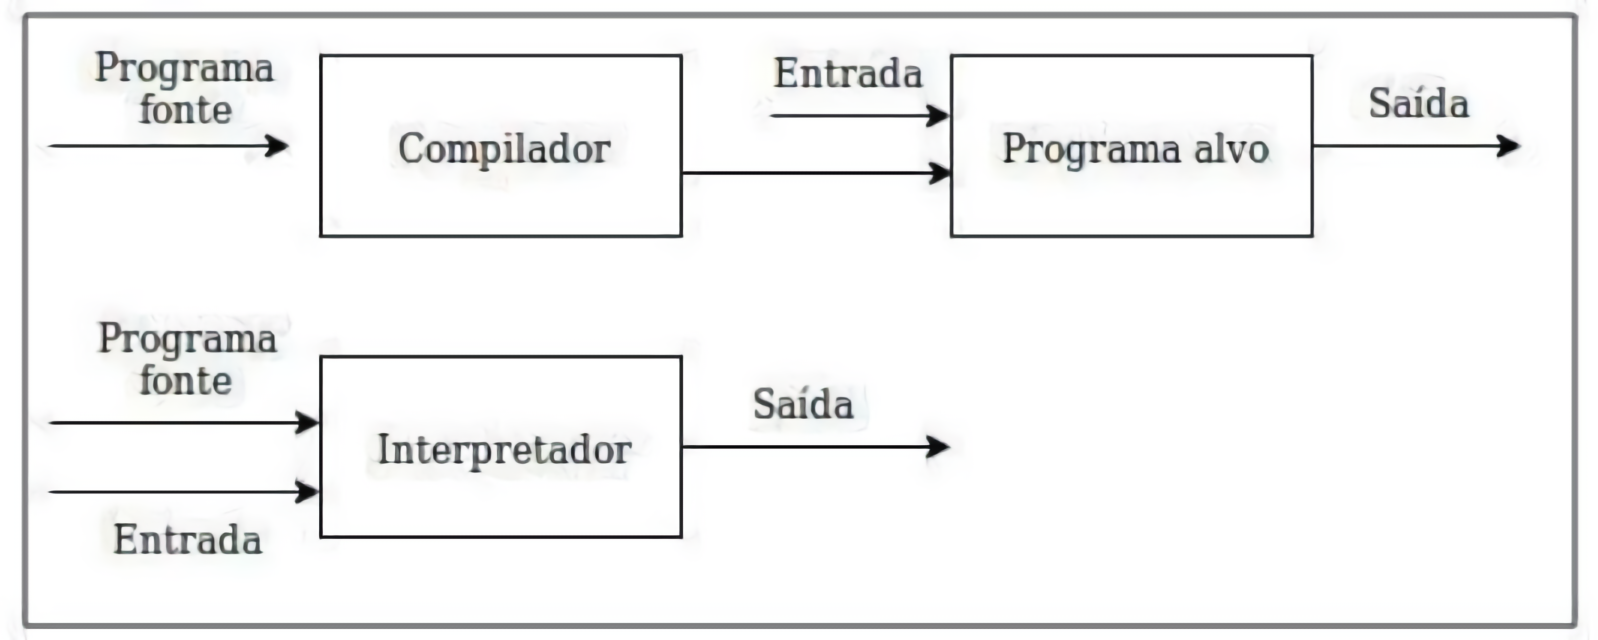
\includegraphics[width=1\textwidth]{img/Cap2/compilador_interpretador.png}
    \caption{Diferença entre compiladores e interpretadores \cite{Miotto2019}}
    \label{fig:compilador_interpretador}
\end{figure}


\subsection{Python}
Python é uma linguagem de programação de propósito geral 
e multiparadigma lançada originalmente em 1991 por Guido van Rossum, estando atualmente em sua terceira versão. Sendo uma linguagem de alto nível, sua filosofia está ligada ao fato de tornar o código mais legível e expressivo, objetivo que é atingido por via de sua sintaxe, muito se assemelhando à linguagem falada. Possui diversas estruturas de alto nível de maneira nativa, como listas, dicionários, data/hora, complexos, dentre outros \cite{Borges2010}, além de ser extensível com o uso de bibliotecas e \emph{frameworks} de terceiros. 

Possui código aberto, significando que Python pode ser livremente usado e modificado por qualquer pessoa. Com isso, a comunidade em volta da linguagem é bem expressiva e engajada. Bibliotecas e \emph{frameworks} possuem forte suporte e costumam ser bem documentados.

\subsection{Solidity}
Solidity é uma linguagem de alto nível orientada a contrato. Ela é utilizada para a implementação de contratos inteligentes (\emph{smart contracts}), sendo atualmente a principal linguagem da plataforma Ethereum \cite{Dannen2017-eb}. É realizada uma compilação a partir dos códigos gerados nessa linguagem a fim de se implantar um contrato inteligente em uma rede Blockchain.

Criada por Gavin Wood, é uma linguagem explicitamente feita para a escrita de contratos inteligentes com funcionalidades a dar suporte direto à execução em ambientes descentralizados Ethereum \cite{Antonopoulos2018-jt}.

\section{Bibliotecas e \emph{frameworks}}

Uma biblioteca é uma coleção de recursos (arquivos, classes, funções) disponível a ser utilizada em um ambiente de programação de computadores. Para \cite{Sommerville2011}, bibliotecas são consideradas como uma questão de implementação no projeto de desenvolvimento de um software. Uma destas questões é o reúso de código fonte já existente. Por se tratar de uma coleção de recursos, programadores podem optar por utilizar bibliotecas prontas ao invés de necessitar implementar as funcionalidades necessárias de um determinado domínio, poupando assim tempo e esforço.

\emph{Frameworks}, por sua vez, são coleções de classes abstratas e concretas que são adaptadas e estendidas para criar sistemas de aplicação \cite{Sommerville2011}. Costumam possuir uma ou mais bibliotecas, além de serem a estrutura mínima necessária para a implementação de projetos diversos. Podem ser vistos como uma espécie de "miniarquitetura" reutilizável que serve como base para e a partir da qual outros padrões de projeto podem ser aplicados \cite{Pressman2021-jj}. \emph{Frameworks} possibilitam a integração, por meio de código, de outros elementos, para a implementação de funcionalidades específicas.

\subsection{Flask}
Flask é um \emph{framework} destinado à web escrito na linguagem de programação Python. Costuma ser chamado de \emph{microframework} pois não necessita de bibliotecas ou ferramentas específicas por padrão. Isto dá uma grande liberdade ao programador, que possui autonomia de implementar suas soluções sem se prender a padrões intrínsecos reforçados por outros \emph{frameworks}.

O \emph{framework} foi projetado desde o seu início para ser extensível, fornecendo um núcleo robusto que inclui funcionalidades básicas necessárias por todas as aplicações baseadas no ecossistema web \cite{Grinberg2018-nz}. Não possui nativamente suporte para acessar bancos de dados, validar formulários, autenticação de usuários, dentre outras tarefas de alto nível \cite{Grinberg2018-nz}. Para isso, são utilizadas extensões fornecidas pela comunidade, que se integram transparentemente com o núcleo do \emph{framework}.

\section{Docker}
O Docker é um mecanismo de conteinerização de código aberto, que automatiza o empacotamento, envio e implantação de quaisquer aplicativos de software \cite{Raj2015-ju}. Em termos práticos, Docker é uma ferramenta que emprega virtualização a nível de sistema operacional, isolando aplicações em estruturas chamadas de contêineres; isto garante que as aplicações sejam executadas de forma isolada, agregando as dependências necessárias dentro do próprio contêiner (como expresso na Figura \ref{fig:docker_diagrama}), evitando assim problemas provenientes de conflitos de versões de bibliotecas.

O Docker foi construído em cima do kernel do sistema operacional Linux, garantindo assim acesso às suas principais funcionalidades, o que promove uma alta eficiência em seu gerenciamento de contêineres. O uso de \emph{namespaces} e \emph{cgroups} dá ao Docker uma alta capacidade de isolar recursos globais do sistema uns dos outros \cite{Raj2015-ju}. Um contêiner Docker é formado a partir de uma imagem Docker. Uma imagem é uma coleção de todos os arquivos que juntos formam uma aplicação de \emph{software}.

\begin{figure}
    \centering
    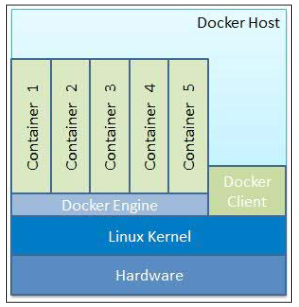
\includegraphics[width=0.45\textwidth]{img/Cap2/Docker Diagrama.png}
    \caption{Demonstração do funcionamento do Docker \cite{Raj2015-ju}}
    \label{fig:docker_diagrama}
\end{figure}

\section{API REST}
REST, acrônimo para \emph{Representational State Transfer} é o nome de um estilo arquitetural para a web elaborado por Roy Fielding em sua dissertação de Ph.D. \cite{Masse2011-cf}. Nela, Fielding detalhou seis características necessárias para sua arquitetura \cite{Grinberg2018-nz}:

\begin{itemize}
    \item \textbf{Modelo Cliente-Servidor}, havendo uma separação distinta entre o papel dos envolvidos;
    \item \textbf{Interface uniforme}, os meios de comunicação nos quais o cliente usa para obter recursos deve ser padronizado, consistente e bem definido;
    \item \textbf{Sistema em camadas}, em que servidores intermediários podem ser utilizados a fim de melhoras na performance, confiabilidade e escalabilidade;
    \item \textbf{Cache}, as respostas do servidor podem estar categorizadas como dados armazenáveis em cache ou não, otimizando a performance dos clientes;
    \item \textbf{\emph{Stateless}} (sem estado), um cliente deve conter toda informação relevante necessária para executar a requisição, tirando a obrigatoriedade do servidor de memorizar o estado de todos os seus clientes;
    \item \textbf{Código sob demanda}, os clientes são capazes de obter código fonte diretamente do servidor e executá-los em seu próprio contexto.
\end{itemize}

Clientes utilizam de APIs (\emph{application programming interface}) para se comunicar com serviços web. Uma API provê um conjunto de funcionalidades para facilitar a troca de informação. Uma API Web em conformidade com o estilo arquitetural REST é uma REST API \cite{Masse2011-cf}. Para ter acesso a recursos, os clientes de uma aplicação recorrem a \emph{URIs} (\emph{Uniform Resource Identifiers}, ou Identificadores Universais de Recursos), que provê uma identificação única a um determinado conceito requisitado pelo usuário \cite{Masse2011-cf}.

\section{Blockchain}

Antes de adentrar o vasto assunto que é Blockchain, devemos definir o que são registros distribuídos. DLTs (do inglês \emph{Distributed Ledger Technology}, Tecnologia de Registro Distribuído) são uma forma de armazenamento em que novas transações podem apenas ser agregadas na estrutura de dados, enquanto que transações antigas não podem ser excluídas ou modificadas \cite{Xu2019-qi}. A Blockchain, por sua vez, é um tipo específico de DLT, consistindo em blocos de dados interligados por meio de criptografia. Um Sistema  Blockchain é definido por \cite{Xu2019-qi} como:
\begin{enumerate}
    \item uma rede blockchain de máquinas, os chamados nós;
    \item uma estrutura de dados para dar suporte às transações e ser replicada aos demais nós na rede;
    \item um protocolo de rede que define e formaliza métodos de interconexão e intercomunicação entre todos os nós da rede, incluindo meios de verificação, validação e consenso.
\end{enumerate}
\cite{Tapscott2016} lista sete princípios fundamentais para uma rede Blockchain:
\begin{enumerate}
    \item \textbf{Integridade na rede}, definida como honestidade nas próprias palavras e atos.
    \item \textbf{Poder distribuído}, a partir do fato de não haver nenhum ponto central detentor do controle sobre toda a rede.
    \item \textbf{Valor como incentivo}, ou o incentivo de participação na rede, gerando recompensas àqueles que contribuem positivamente na comunidade.
    \item \textbf{Segurança}, por meio da obrigação do uso de criptografia e a responsabilização daqueles que agem de má fé dentro da rede.
    \item \textbf{Privacidade}, a capacidade dos usuários da rede de deter controle de seus próprios dados e a eliminação da necessidade de conhecer a verdadeira identidade daqueles que interagem na rede.
    \item \textbf{Direitos preservados}, a necessidade de se respeitar liberdades individuais.
    \item \textbf{Inclusão}, reduzir os obstáculos no processo de participação.
\end{enumerate}

A tecnologia Blockchain foi originalmente concebida por Satoshi Nakamoto em um artigo ao propor a moeda digital Bitcoin. Apesar de criar a base da tecnologia, Satoshi não chegou a cunhar a palavra “Blockchain” \cite{nakamoto2009bitcoin}, termo que se popularizou apenas anos mais tarde. É uma rede pública ponto a ponto em que qualquer pessoa pode participar. Suas principais características são o fato de utilizar criptografia e ser uma rede distribuída. Cada bloco de uma Blockchain possui um identificador único, chamado de \emph{hash}, que é calculado a partir dos dados contidos em cada bloco. Além de seu próprio \emph{hash}, também armazena o \emph{hash} do bloco anterior, formando a cadeia de blocos propriamente dita. Na eventualidade de um agente malicioso alterar os dados de uma transação, o \emph{hash} do bloco em questão mudará, acarretando uma mudança no \emph{hash} de seu sucessor, e assim sucessivamente até o último bloco da cadeia. Um cliente desta rede, ao observar este estado de inconsistência, certamente optará por não utilizar os dados pois deduz-se que houve uma adulteração na rede.

A etapa de mineração de um bloco é igualmente importante para a rede. Como a Blockchain se firma na ideia de descentralização, sua integridade é garantida por um acordo mútuo entre vários de seus usuários, formando um consenso. Para atingir o consenso usam-se algoritmos, sendo o mais usado o chamado Prova de Trabalho (\emph{Proof of Work}, PoW), em que a validação de um bloco consiste em resolver um problema matemático de difícil solução. A rede é dependente da figura do minerador, que tem o papel de agregar as transações válidas em blocos e as unir na Blockchain \cite{Xu2019-qi}. Devido aos altos custos operacionais de concretizar a resolução deste problema, sobretudo tempo e energia, o primeiro nó a achar a resposta é definido como o criador do bloco e recebe uma quantia em criptomoeda como recompensa pelo seu trabalho. O papel fundamental da mineração é dar seguridade à Blockchain ao tempo em que o controle é mantido de forma difusa e descentralizada pela maior quantidade de participantes possíveis \cite{Antonopoulos2018-jt}.

Outra abordagem para garantir o consenso é a utilização da Prova de Participação (\emph{Proof of Stake}, PoS). Nela, a blockchain gerencia um conjunto de validadores que podem "investir" quantias de criptomoeda da própria Blockchain para tentar validar o bloco. A quantia é depositada e permanece isolada até o fim do processo de validação. Os validadores, então, se revezam em uma votação, em que os pesos dos votos são determinados diretamente pela quantia depositada. A abordagem tomada por este método garante que os validadores bem intencionados recebam de volta a quantia de criptomoeda investida e recebam adicionalmente uma quantia proporcional à sua participação, ao passo que aqueles que agirem de má fé são punidos com a não devolução de sua quantia de criptomoeda \cite{Antonopoulos2018-jt}. A Prova de Participação foi concebida levando em consideração o quão custosa é a Prova de Trabalho, tomada como dispendiosa devido aos altos custos envolvidos com energia elétrica, necessária para realizar os cálculos computacionais para validação.

Na hipótese de uma pessoa tentar roubar uma unidade de Bitcoin, ela teria que reescrever todo o histórico de transações da rede \cite{Tapscott2016} e então transmitir suas alterações aos demais nós, o que seria computacionalmente inviável. Como as transações da rede sofrem broadcast para a rede, todos os pares da rede podem verificar sua validade \cite{Karame2016-qb}.

O Bitcoin originalmente se propôs a resolver o problema do gasto duplo por meio de redes peer to peer \cite{nakamoto2009bitcoin}, se firmando posteriormente como uma excelente solução na área de pagamentos e transferência de dinheiro por vias digitais. Na plataforma Ethereum, uma transação consiste no ato de persistir dados na Blockchain utilizando uma assinatura eletrônica concebida a partir de uma conta originária, realizando o envio até um endereço específico dentro da rede. A transação é composta por metadados tais como os campos \emph{sender}, \emph{recipient}, \emph{value} e \emph{data payload} \cite{Antonopoulos2018-jt}. Para assinar transações, os usuários necessitam de uma chave criptográfica privada correspondente à sua conta; esta conta, por sua vez, é definida como uma chave pública. A chave privada é um dado sensível pois prevê um acesso total aos recursos da conta, cabendo ao usuário guardá-la com segurança. Uma solução é utilizar uma carteira, um software que permite seus usuários gerenciarem uma coleção de chaves privadas. As carteiras funcionam como uma espécie de nó parcial do Blockchain, guardando apenas transações resultantes das contas salvas \cite{Xu2019-qi}. A privacidade dos usuários de uma Blockchain advém do uso de pseudônimos, os endereços públicos \cite{Karame2016-qb}.

\subsection{Contratos inteligentes}
O termo \emph{Smart Contract} foi cunhado pelo criptógrafo Nick Szabo na década de 1990 \cite{Antonopoulos2018-jt}. Embora Szabo tenha definido o termo originalmente como um conjunto de promessas em formato digital sustentadas por meio de protocolos, o conceito evoluiu e passou a ter maior abrangência. \cite{Xu2019-qi} define contratos inteligentes como programas implantados em registros de uma Blockchain que são executados por meio de transações, sendo capazes de manter e transferir recursos digitais gerenciados pela própria Blockchain. São capazes de executar outros contratos e, tal como os registros salvos na rede, são imutáveis.

Contratos inteligentes em Ethereum não devem ser vistos como representações de contratos legais que devem ser cumpridos, em vez disso, são mais similares a agentes que podem ser invocados dentro de um ambiente de execução Ethereum \cite{Xu2019-qi}. Um exemplo de implantação de contrato inteligente na rede está expresso na Figura \ref{fig:contrato_inteligente}.


\subsection{Plataforma Ethereum}
Ethereum é uma Blockchain aberta e descentralizada lançada originalmente em 2015, sua criptomoeda é chamada de Ether, denotado com as letras ETH. Foi criada com o intuito de ser um protocolo alternativo para a criação de aplicações descentralizadas. Ethereum buscou implementar aspectos não tratados pela plataforma Bitcoin, como a falta de suporte a uma linguagem Turing-completa, estados e value/blockchain-awareness (conscientização de dados) \cite{Buterin2013}. A implantação (\emph{deployment}) de contratos inteligentes é possível com o uso da \emph{Ethereum Virtual Machine} (EVM), uma máquina virtual encarregada de compilar códigos oriundos de linguagens de programação de alto nível em bytecode, ou instruções em código de máquina; cada um dos bytes representa uma operação \cite{Buterin2013}. Para realizar comunicação com os contratos, vem à tona o conceito de ABI (\emph{Application Binary Interface}), que nada mais é do que uma interface ou meio de comunicação entre duas entidades; cada contrato possui um ABI próprio, que define os métodos disponíveis. Um ABI possibilita interações de contrato-contrato ou aplicação-contrato \cite{eiki_2019}.

\begin{figure}
    \centering
    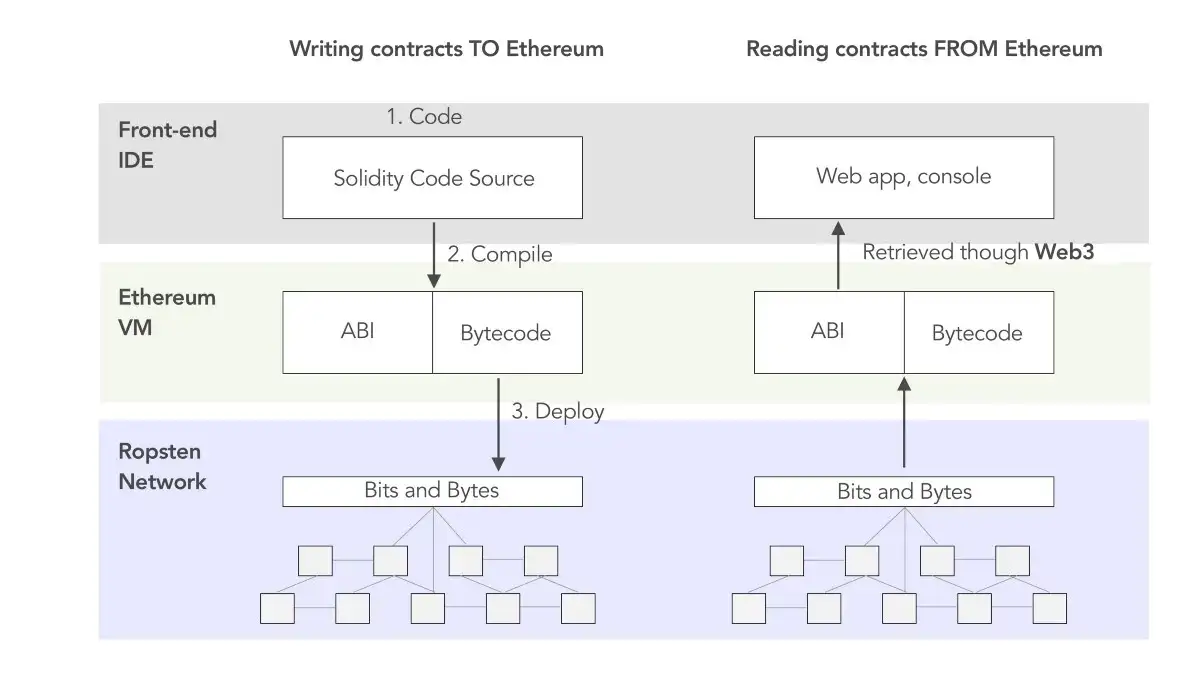
\includegraphics[width=1\textwidth]{img/Cap2/ethereum contracts.png}
    \caption{Implantação de um contrato inteligente em uma \emph{testnet} \cite{eiki_2019}}
    \label{fig:contrato_inteligente}
\end{figure}

Devido ao seu suporte de linguagens Turing-completas, a plataforma Ethereum abre margem para certos problemas computacionais \cite{Antonopoulos2018-jt}: por definição, um programa de computador Turing-completo é incapaz de prever seu fluxo de execução. Em outras palavras, é impossível um algoritmo saber quando sua execução irá terminar \cite{Sipser2012-gl}. Portanto, cenários em que execuções muito longas ocorrem, tal como a execução repetida de um mesmo trecho de código em um número exorbitante de vezes (os chamados loops infinitos), são imprevisíveis. Em um ambiente de execução distribuído, isto pode alavancar consequências indesejáveis, sobretudo desperdício de recursos computacionais e problemas de desempenho nos nós pertencentes a esse sistema. 
Para tratar deste problema, a plataforma Ethereum implementa um mecanismo chamado gas. Ao executar um contrato inteligente na EVM, cada comando do contrato invoca instruções do processador da máquina utilizada, como somar dois valores e persistir um dado. A partir daí, realiza-se um cálculo de gas com base no número de instruções utilizadas para efetuar a transação. Cada transação enviada deve conter obrigatoriamente um limite máximo de gas que está disposta a consumir para concretizar a operação. Se a quantidade de gas consumido exceder a quantidade de gas disponível, a execução do contrato é terminada. Desta forma, a rede garante limites para o uso de recursos computacionais, prevenindo abusos e gastos desnecessários. O gas é obtido com o uso da criptomoeda Ether \cite{EthereumGas}.

 Para realizar transações na rede, são utilizados valores fracionados da moeda Ether. Isso ocorre devido ao alto valor da criptomoeda: na primeira semana de fevereiro de 2023 a cotação de um único Ether era, em média, R\$ 8.400,00, o que equivale a aproximadamente US\$ 1.630,00. Devido ao valor diminuto de Ether necessário para realizar transações, foram criadas subdivisões para diferentes escalas da moeda, cada uma delas possuindo um nome padronizado pelo SI (Sistema Internacional de Unidades) junto de nomes coloquiais, fazendo homenagem a grandes pesquisadores da área de computação e da criptografia \cite{Antonopoulos2018-jt}. A menor unidade da criptomoeda é o \emph{wei}, sendo também o valor base utilizado na rede descentralizada.

 \begin{table}[H]
 \centering
\begin{tabular}{llll}
\hline
\multicolumn{1}{|l|}{Valor em wei} & \multicolumn{1}{l|}{Magnitude} & \multicolumn{1}{l|}{Nome coloquial} & \multicolumn{1}{l|}{Nome no SI} \\ \hline
\multicolumn{1}{|l|}{1} & \multicolumn{1}{l|}{1} & \multicolumn{1}{l|}{wei} & \multicolumn{1}{l|}{Wei} \\ \hline
\multicolumn{1}{|l|}{1,000} & \multicolumn{1}{l|}{10\textasciicircum{}3} & \multicolumn{1}{l|}{Babbage} & \multicolumn{1}{l|}{Kilowei/femtoether} \\ \hline
\multicolumn{1}{|l|}{1,000,000} & \multicolumn{1}{l|}{10\textasciicircum{}6} & \multicolumn{1}{l|}{Lovelace} & \multicolumn{1}{l|}{Megawei/picoether} \\ \hline
\multicolumn{1}{|l|}{1,000,000,000} & \multicolumn{1}{l|}{10\textasciicircum{}9} & \multicolumn{1}{l|}{Shannon} & \multicolumn{1}{l|}{Gigawei/nanoether} \\ \hline
\multicolumn{1}{|l|}{1,000,000,000,000} & \multicolumn{1}{l|}{10\textasciicircum{}12} & \multicolumn{1}{l|}{Szabo} & \multicolumn{1}{l|}{Microether} \\ \hline
\multicolumn{1}{|l|}{1,000,000,000,000,000} & \multicolumn{1}{l|}{10\textasciicircum{}15} & \multicolumn{1}{l|}{Finney} & \multicolumn{1}{l|}{Milliether} \\ \hline
\multicolumn{1}{|l|}{1,000,000,000,000,000,000} & \multicolumn{1}{l|}{10\textasciicircum{}18} & \multicolumn{1}{l|}{Ether} & \multicolumn{1}{l|}{Ether} \\ \hline
 &  &  &  \\
 &  &  &     
\end{tabular}
\caption{Valores monetários da criptomoeda Ether}
    \label{tab:tabela_valores_ether}
\end{table}


\subsection{\emph{Testnet}}
Abreviação de \emph{test network}, é uma rede utilizada para simular o comportamento da rede principal da plataforma Ethereum \cite{Antonopoulos2018-jt}. Como são redes paralelas, as \emph{testnets} são utilizadas para a realização de testes diversos, como transações, implantação e depuração de contratos antes destes serem migrados para a rede principal. As criptomoedas de uma \emph{testnet} não possuem valor real e podem ser facilmente adquiridas por via de \emph{faucets} (torneiras) de ether \cite{Dannen2017-eb}, servidores que transferem ether de teste à uma conta de uma \emph{testnet}.

\section{Segurança da Informação}
Os pilares da segurança de informação se baseiam na chamada tríade CIA (do inglês \emph{confidentiality}, \emph{integrity} e \emph{availability}). \cite{Nakamura2016} afirma que todas essas propriedades devem ser protegidas como um todo, e não isoladamente.

\begin{itemize}
    \item \textbf{Confidencialidade}: restringir dados e informações confidenciais a entidades não autorizadas. Também engloba a noção de privacidade, dando a estas entidades a autonomia de saber como, quais são e por quem seus dados estão sendo utilizados e de decidir se suas informações poderão ser acessadas, perante consentimento.
    \item \textbf{Integridade}: garantir que as informações transmitidas e armazenadas dentro do sistema não sofram nenhum tipo de adulteração, permitindo alterações somente a entidades previamente autorizadas.
    \item \textbf{Disponibilidade}: garantir que o sistema computacional consiga operar de forma normal e ininterrupta, sem haver nenhum tipo de inatividade que prejudique seus usuários.
\end{itemize}

Defronte destas definições, \cite{Stallings2015} vai além e lista adicionalmente os conceitos de autenticidade e responsabilização:
\begin{itemize}
    \item \textbf{Autenticidade}: a capacidade de uma entidade ser verificada e confiável, promovendo seguridade em meio a uma transação. Com ela conseguimos averiguar a identidade da entidade comunicante e saber se ela advém de uma fonte confiável ou não
    \item \textbf{Responsabilização}: a capacidade de figurar dentro de um sistema computacional os indivíduos responsáveis por suas ações, provendo assim irretratabilidade e meios de averiguar as transações realizadas. É necessária pois sistemas totalmente seguros ainda não são uma realidade.
\end{itemize}

\subsection{Criptografia}
A área de criptografia é constituída pelos muitos esquemas utilizados para encriptação de uma mensagem \cite{Stallings2015}. O processo de cifração consiste em transformar uma mensagem originalmente inteligível em uma mensagem cifrada por meio de uma série de substituições e transformações com o uso de um algoritmo. Blockchains usam as chamadas funções de \emph{hash} em seu funcionamento. Funções de \emph{hash} são funções que recebem uma determinada informação de entrada e produzem como saída uma cifra única dentro de sua capacidade (espaço de chaves). Em especial, usa-se a função SHA-256 da família de funções \emph{Secure Hash Algorithm} para produzir identificadores únicos na Blockchain, também chamados de endereços, que agem como uma assinatura digital de cada bloco da rede. Uma característica essencial das funções de \emph{hash} é a resistência a colisão, uma propriedade que garante que é computacionalmente inviável achar duas entradas distintas que resultem em um mesmo \emph{hash}. Esta propriedade constitui um dos pilares de segurança da Blockchain \cite{Karame2016-qb}.

\section{\emph{Logs}}
Um \emph{log} é uma mensagem gerada pelo sistema em resposta a algum tipo de estímulo \cite{Chuvakin2013-za}. Estes estímulos dependem do contexto e podem ser diversos, indo desde o simples login de um usuário em um ambiente Unix até mensagens de falha de hardware. O termo \emph{logs} costuma ser usado para expressar uma coleção de mensagens de \emph{log} referentes a um determinado uso. Podem ser armazenadas de diferentes maneiras, como arquivos de texto ou tabelas em um banco de dados relacional. Mensagens podem ser classificadas como:

\begin{itemize}
    \item \textbf{Informacionais}, projetadas para comunicar a usuários e administradores de algum acontecimento benigno;
    \item \textbf{Debug}, implantadas em sistemas de software com o intuito de auxiliar desenvolvedores de software a identifiar problemas com a aplicação;
    \item \textbf{Aviso}, usada em situação em que recursos podem estar faltando mas não são explicitamente necessários para o funcionamento do sistema;
    \item \textbf{Erro}, usada para notificar erros diversos que podem ocorrer em um sistema
    \item \textbf{Alerta}, utilizado para indicar o acontecimento de algo de interesse no sistema.
\end{itemize}

Cada mensagem de \emph{log} deve conter os seguintes elementos básicos: \emph{timestamp}, fonte e dados. Independente de como são armazenadas, as mensagens deverão conter estes itens. A \emph{timestamp} diz respeito a quando a mensagem foi gerada. A fonte, tipicamente um endereço IP ou \emph{hostname}, se refere ao sistema que gerou a mensagem de \emph{log}. Os dados são referentes à informação em si que o sistema deseja persistir, não possuindo padronização e nem representação fixa \cite{Chuvakin2013-za}.

\section{Auditoria}
Segundo \cite{Chuvakin2013-za}, auditoria é um processo que verifica se um sistema ou processo está funcionando como esperado. São chamados de auditores aqueles que realizam tarefas de auditoria, sendo responsáveis pelo bom funcionamento de controles internos \cite{Champlain2003-za} de empresas e organizações com o objetivo de mitigar riscos. Os auditores atuam aplicando julgamentos baseados em experiência e conhecimento para gerenciar os riscos possíveis em um contexto organizacional. O ideal é que todas as organizações passem por avalizações de risco e implementem maneiras de lidar com possíveis incidentes. A necessidade por auditoria sempre existiu, mas a sua urgência tem aumentado \cite{Champlain2003-za}, sobretudo por conta de ataques cibernéticos.

\emph{Logs} integram parte do processo de auditoria, implementando políticas de não repúdio (ou irretratabilidade) por meio das chamadas trilhas de auditoria. Uma trilha de auditoria é o registro de todas as ações realizadas por uma entidade em um sistema. Desta forma, toda e qualquer ação que seja executada em uma aplicação terá a garantia de que estará embasada e vinculada a um determinado usuário, atribuindo-lhe a responsabilidade pelo ato cometido. 

Define-se como trilha de auditoria um registro de todas as ações, eventos ou atividades realizadas por um usuário em um sistema \cite{privacytech_2020}. Englobam-se operações como criação de registros, bem como modificação e exclusão. Devido ao possível alto número de registros gerados numa base diária em um sistema, deve-se empregar técnicas para um rastreamento preciso e eficaz.

Segundo \cite{privacytech_2020}, a trilha de auditoria pode ser usada para diferentes finalidades:

\begin{itemize}
    \item Segurança da informação - a partir da trilha de auditoria é possível identificar que algo de errado aconteceu no sistema. Isto é possível por meio do armazenamento e rastreio de atividades de ações.

    \item Conformidade regulamentar - para dar a garantia de que o sistema é seguro e de que está em conformidade com normas e regulamentos diversos.

    \item Análise forense digital - a possibilidade de descobrir quem e porquê realizou determinada ação, com a capacidade de provar que a entidade responsável realmente realizou a ação.

    \item Integridade dos dados - a trilha de auditoria permite a reconstrução de dados que foram modificados e a hora em que foram modificados.

    \item Análise de negócios - os \emph{logs} fornecem uma visão geral acerca do funcionamento do negócio, já que a trilha de auditoria contém os dados que refletem diretamente aos processos do negócio.

    \item Detecção de fraudes e anomalias - devido à coleta de \emph{logs}, é possível a identificação de fraudes e anomalias ocorridas no sistema.
\end{itemize}


\section{Teste de \emph{software}}
Teste de \emph{software} é a prática de validar que o comportamento de uma aplicação seja aquilo que se espera \cite{Mohan2022-ch}. \cite{Pressman2021-jj}, por sua vez, define teste como um conjunto de atividades que podem ser planejadas com antecedência e executadas sistematicamente. A utilidade do teste de \emph{software} no processo de desenvolvimento é garantir qualidade ao código produzido. Não existe garantia de que todo \emph{software} seja totalmente livre de erros, então tem-se a necessidade de testar artefatos de \emph{software} para identificar possíveis erros inseridos durante sua construção.

Dois dos principais métodos de teste de \emph{software} são o teste de caixa-branca e o teste de caixa-preta. O teste de caixa-branca, também conhecido como teste estrutural, é uma abordagem de testes em que detalhes de implementação do código-fonte são conhecidos e estruturas internas do \emph{software} são testadas. Fluxos de controle costumam ser um dos focos desta abordagem. O teste de caixa-preta, também chamado de teste funcional, tem por foco os requisitos funcionais do \emph{software} \cite{Pressman2021-jj}. A partir de diferentes dados de entrada obtém-se diferentes tipos de saídas, que são validadas com base nos requisitos da aplicação. As técnicas de caixa-branca e caixa-preta não são mutuamente exclusivas, ambas têm diferentes focos de teste e se complementam.

Existem diversos tipos de testes que podem ser realizados em um sistema, possuindo diferentes escopos e aplicabilidades. Dois deles são foco deste trabalho: testes de unidade e testes de integração. Os testes de unidade se baseiam em testar as menores unidades de um sistema, que pode ser um método, uma função ou um componente, e garantir que ele funcione adequadamente. Já os testes de integração se referem a testes que são direcionados a sistemas que possuem diferentes módulos interagindo entre si. Mesmo que cada um dos módulos funcione de maneira correta individualmente, sua conjunção pode apresentar falhas. \cite{Pressman2021-jj} sugere que isto ocorre devido a falhas de interfaces, que podem ocasionar perda de dados, consequentemente acarretando em comportamentos inesperados em todo o conjunto de \emph{software}.
\chapter{Desenvolvimento}
Este capítulo terá como foco detalhar o sistema proposto, apresentar sua modelagem e comentar seus aspectos técnicos e funcionais. Serão apresentados os requisitos funcionais e não funcionais, obtidos por meio de análise de requisitos, nos quais a implementação tomou como base, além de mostrar diagramas UML que fundamentam diferentes aspectos do sistema. \cite{Sommerville2011} define o estágio de desenvolvimento sendo composto por todas as atividades envolvidas no desenvolvimento do sistema, como definição de requisitos, projeto de sistemas, engenharia de hardware e software, integração de sistemas e testes.

O \emph{software} implementado se baseou nas principais práticas de engenharia de \emph{software}, tornando o processo de desenvolvimento fluido, adotando o modelo em cascata como metodologia de desenvolvimento.

\section{Descrição geral}
O sistema implementado é uma API REST visando manter um registro de todas as ações tomadas pelo usuário do aplicativo Carteira Digital do Restaurante Universitário da UEA (APP-RU). O sistema é uma solução proposta à problemática de salvar dados de alunos de forma segura, utilizando a Blockchain como meio de persistir informações de forma íntegra e privativa. Com isto, logs do tipo informacional são guardados na rede distribuída. A partir de requisições, a API REST processa o pedido do usuário, captando os dados necessários para realizar um registro da ação executada na plataforma Ethereum. Exemplificando: se um aluno comprar um ticket, uma requisição é disparada, sendo captada pela aplicação Python e extraindo os dados necessários para persistir os dados na Blockchain, por meio da chamada de um contrato inteligente.

\section{Tecnologias utilizadas}
Para desenvolver o projeto, optou-se pela linguagem de programação Python para criar a API REST e a linguagem Solidity para implementar o contrato inteligente que é executado na plataforma Ethereum. 

De modo a facilitar a execução do código produzido e o processo de implantação do sistema, utilizou-se a tecnologia Docker. As tecnologias e dependências utilizadas neste projeto são:

\begin{table}[H]
    \centering
    \begin{tabular}{ | p{3cm} | p{1.75cm} | p{10cm} |}
        \hline
        \textbf{Biblioteca} & \textbf{Versão} & \textbf{Utilidade}\\
        \hline

        Docker & 20.10.16 & Virtualização de imagens  \\
        \hline

        Python & 3.10 & Linguagem de programação para construção da solução. Disponibilizada via imagem Docker  \\
        \hline

        Flask & 2.2.2 & \emph{Microframework} destinado à construção de APIs  \\
        \hline

        flask-smorest & 0.40.0 & Serialização de dados e geração de documentação da API.  \\
        \hline

        python-dotenv & 0.21.0 & Gerenciamento de variáveis de ambiente  \\
        \hline

        Web3.py & 5.31.3 & Conexão com a Blockchain  \\
        \hline

        Solidity & 0.8 & Desenvolvimento de contratos inteligentes  \\
        \hline
    \end{tabular}
    \caption{Tecnologias utilizadas para o desenvolvimento da solução}
    \label{tab:tecnologias_utilizadas}
\end{table}

A \emph{testnet} usada neste trabalho é a rede Goerli (chamada também de Görli), junto da rede Sepolia. Goerli surgiu em 2019 e é uma das principais redes de teste públicas da plataforma Ethereum, juntamente com a \emph{testnet} Sepolia. Diferentemente de outras redes de teste que se tornaram depreciadas como Ropsten e Rinkeby, Goerli é mantida e desenvolvida pela própria comunidade Ethereum. A rede possui um explorador de transações próprio tal como existe com a \emph{mainnet}, chamado de Goerli Etherscan, que fornece uma interface intuitiva para visualizar dados da Blockchain, como transações efetuadas, contratos implantados e informações sobre determinados blocos da rede.

\section{Modelagem do sistema}
\subsection{Requisitos}

\subsubsection{Requisitos funcionais}
\begin{table}[H]
    \centering
    \begin{tabular}{ | p{3cm} | p{10cm} |}
        \hline
        \textbf{Identificador} & \textbf{Descrição}\\
        \hline

        RF01 & A API REST deverá salvar registros (\emph{logs}) de ações executadas pelo usuário no APP-RU na Blockchain  \\
        \hline
        
        RF02 & Os dados devem ser persistidos na Blockchain por meio do uso de um contrato inteligente implantado na plataforma Ethereum \\
        \hline

        RF03 & A API REST deverá ser capaz de retornar dados referentes ao uso do APP-RU \\
        \hline

        RF04 & A persistência de dados deverá ocorrer por meio do uso do formato de dados \emph{string} na Blockchain \\
        \hline

        RF05 & A API REST deverá ser capaz de registrar em sua mensagem de \emph{log} a data e a hora da realização de uma interação com o APP-RU de um determinado usuário \\
        \hline

        RF06 & A API REST deverá ser capaz de registrar em sua mensagem de \emph{log} o módulo requisitado por um determinado usuário \\
        \hline

        RF06 & A API REST deverá ser capaz de registrar em sua mensagem de \emph{log} uma mensagem referente ao ato realizado por um determinado usuário, junto de sua identificação única \\
        \hline

    \end{tabular}
    \caption{Requisitos funcionais}
    \label{tab:my_label}
\end{table}

\subsubsection{Requisitos não funcionais}
\begin{table}[H]
    \centering
    \begin{tabular}{ | p{3cm} | p{10cm} |}
        \hline
        \textbf{Identificador} & \textbf{Descrição}\\
        \hline
        
        RNF01 & A aplicação local deverá ser executada isoladamente em um contêiner Docker, garantindo assim um melhor gerenciamento de dependências e um processo de implantação mais ágil \\
        \hline
        
        RNF02 & A API REST deverá estar documentada por meio do uso do padrão OpenAPI 3.0 \\
        \hline

        RNF03 & O sistema deverá ser utilizado por meio de requisições à API REST, realizando comunicação com seus clientes com o uso do formato de dados JSON \\
        \hline
        
        RNF04 & O sistema deverá, por meio do uso da Blockchain, garantir confiabilidade, integridade, disponibilidade aos dados trafegados \\
        \hline

        RF05 & A comunicação com a Blockchain se dará com o uso da plataforma Ethereum, devendo ser mediada por meio de um provedor Infura, garantindo estabilidade e robustez nas transações
        \\
        \hline

        RNF06 & O sistema deverá ser de fácil manutenção \\
        \hline

        RNF07 & O sistema deverá ser facilmente extensível, possibilitando a implementação de novas funcionalidades em tempo posterior \\
        \hline

        RNF08 & O sistema deverá ser resiliente a falhas de âmbito interno, não admitindo erros capazes de parar o funcionamento da aplicação \\
        \hline
    \end{tabular}
    \caption{Requisitos não funcionais}
    \label{tab:my_label}
\end{table}

\subsection{Diagrama de Casos de Uso}
\begin{figure}
    \centering
    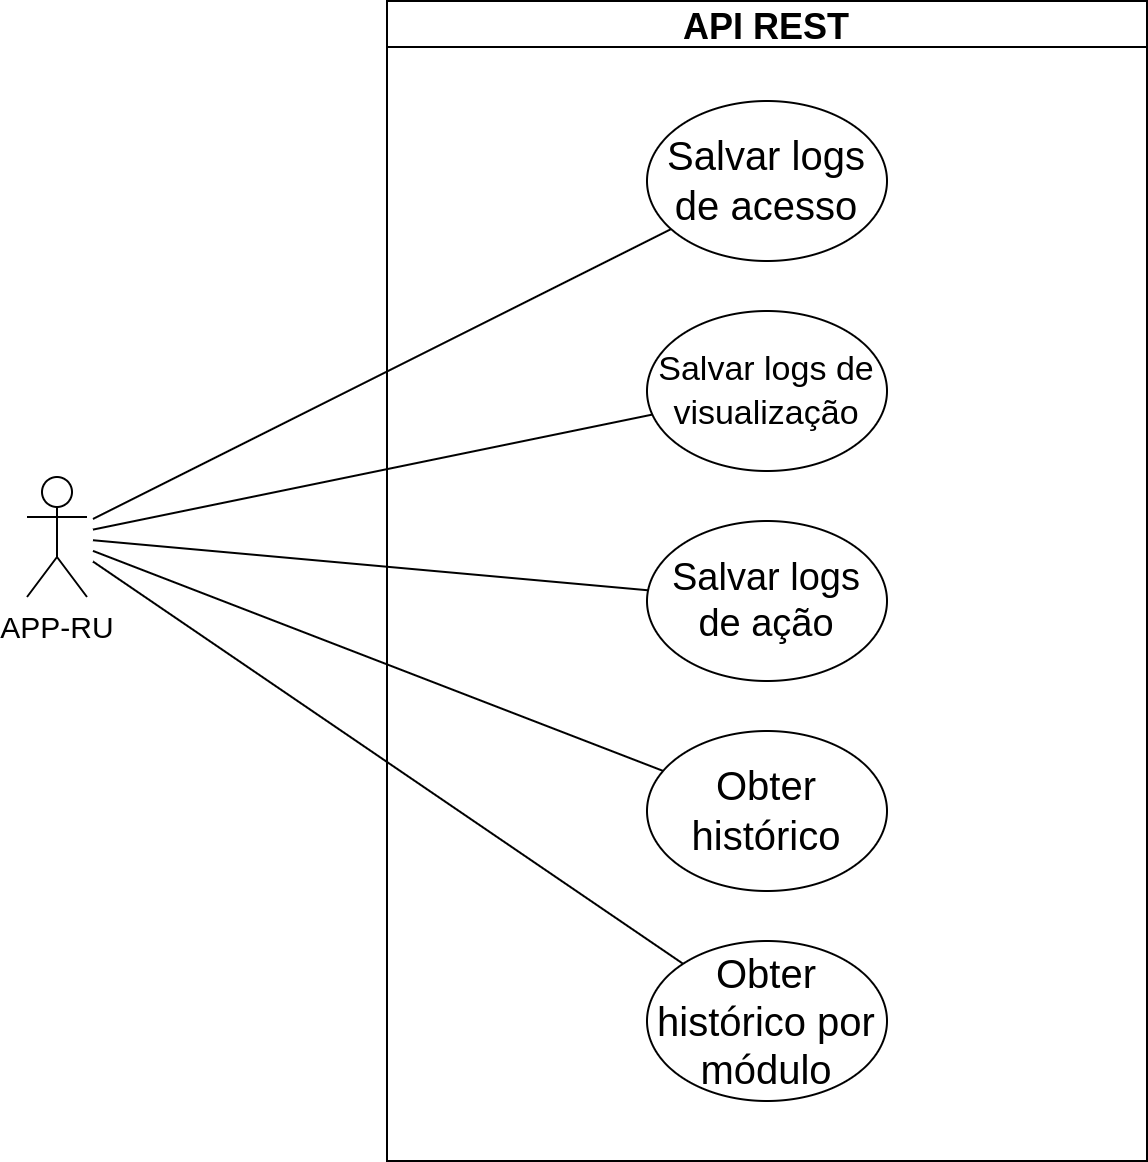
\includegraphics[width=0.75\textwidth]{img/Cap3/diagramas/Diagrama de Casos de Uso.png}
    \caption{Diagrama de Casos de Uso}
    \label{fig:diagrama_casos_uso}
\end{figure}
O papel do Diagrama de Casos de Uso é detalhar quem são os atores, ou seja, as partes envolvidas, e como eles interagem com o sistema. Para \cite{Sommerville2011}, um caso de uso identifica os atores em uma interação e dá nome ao tipo de interação. Os atores podem ser usuários do sistema ou mesmo uma máquina ou um outro sistema.

Neste contexto, um ator é qualquer entidade que faça uso (consuma) da API REST. Em especial, alunos da universidade e administradores do sistema utilizam a API por meio de requisições feitas em seus dispositivos. Outra maneira de de utilizá-la é via uso dos chamados \emph{API Clients}, \emph{softwares} próprios para o envio de requisições que são usados sobretudo em ambientes de desenvolvimento.

O diagrama apresentado na Figura \ref{fig:diagrama_casos_uso} retrata os casos de uso do usuário aluno. Para cada ação realizada pelo aluno, a API disponibiliza um \emph{endpoint} em que são enviados os seus dados. A cada requisição realizada em um \emph{endpoint}, um novo \emph{log} é gerado, sendo posteriormente persistido na plataforma Ethereum.

\newpage
\subsection{Diagrama de Atividades}
\begin{figure}
    \centering
    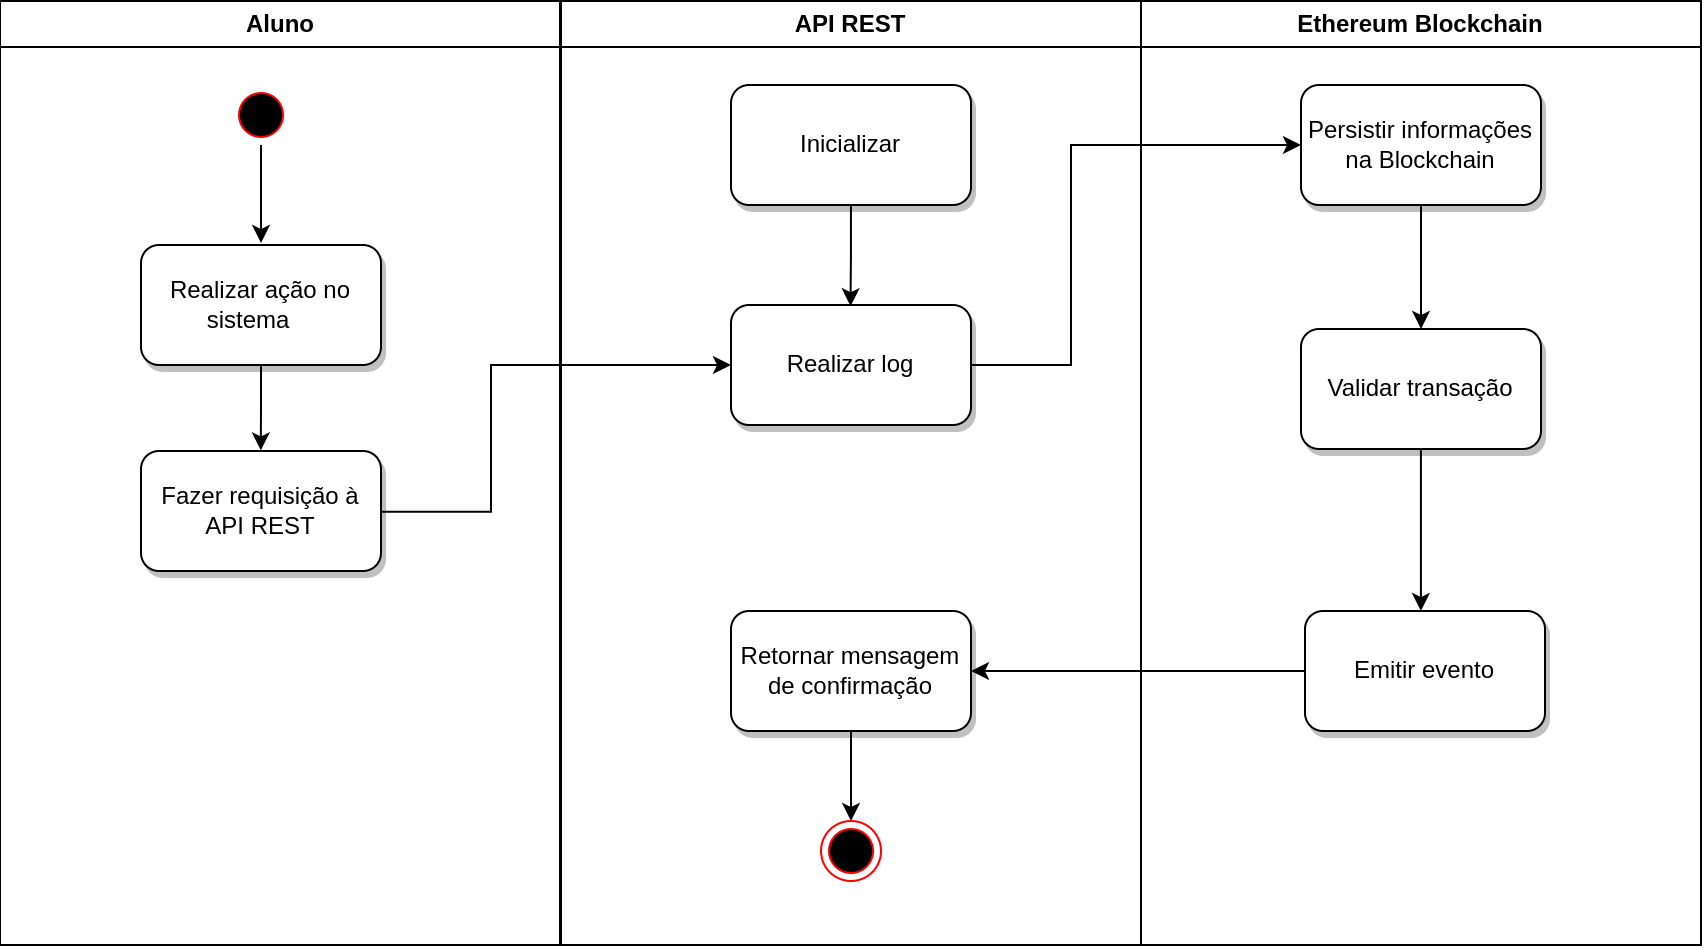
\includegraphics[width=1\textwidth]{img/Cap3/diagramas/Diagrama de Atividade.png}
    \caption{Diagrama de Atividades}
    \label{fig:diagrama_atividades}
\end{figure}
Ao passo em que Diagramas de Casos de Uso detalham o que o sistema deve fazer, os Diagramas de Atividades especificam como o sistema irá alcançar o seu objetivo \cite{Miles2006-fo}. Os Diagramas de Atividades possuem início e fim bem delimitados, representados por círculos preenchidos inseridos no diagrama. Eles exprimem quais são as atividades que compõe um processo dentro do sistema, e o fluxo de controle de uma atividade a outra \cite{Sommerville2011}.

O diagrama aqui apresentado na Figura \ref{fig:diagrama_atividades} ilustra a maneira em que as diferentes partes realizam comunicação para registrar um \emph{log} na plataforma Ethereum. A API REST, após inicializada, recebe uma requisição do usuário e utiliza os dados coletados para realizar uma transação na Blockchain, encarregada de validar esta transação e então emitir um evento à API, concluindo a operação com o envio de uma confirmação ao usuário.

\newpage
\subsection{Diagrama de Sequência}
\begin{figure}
    \centering
    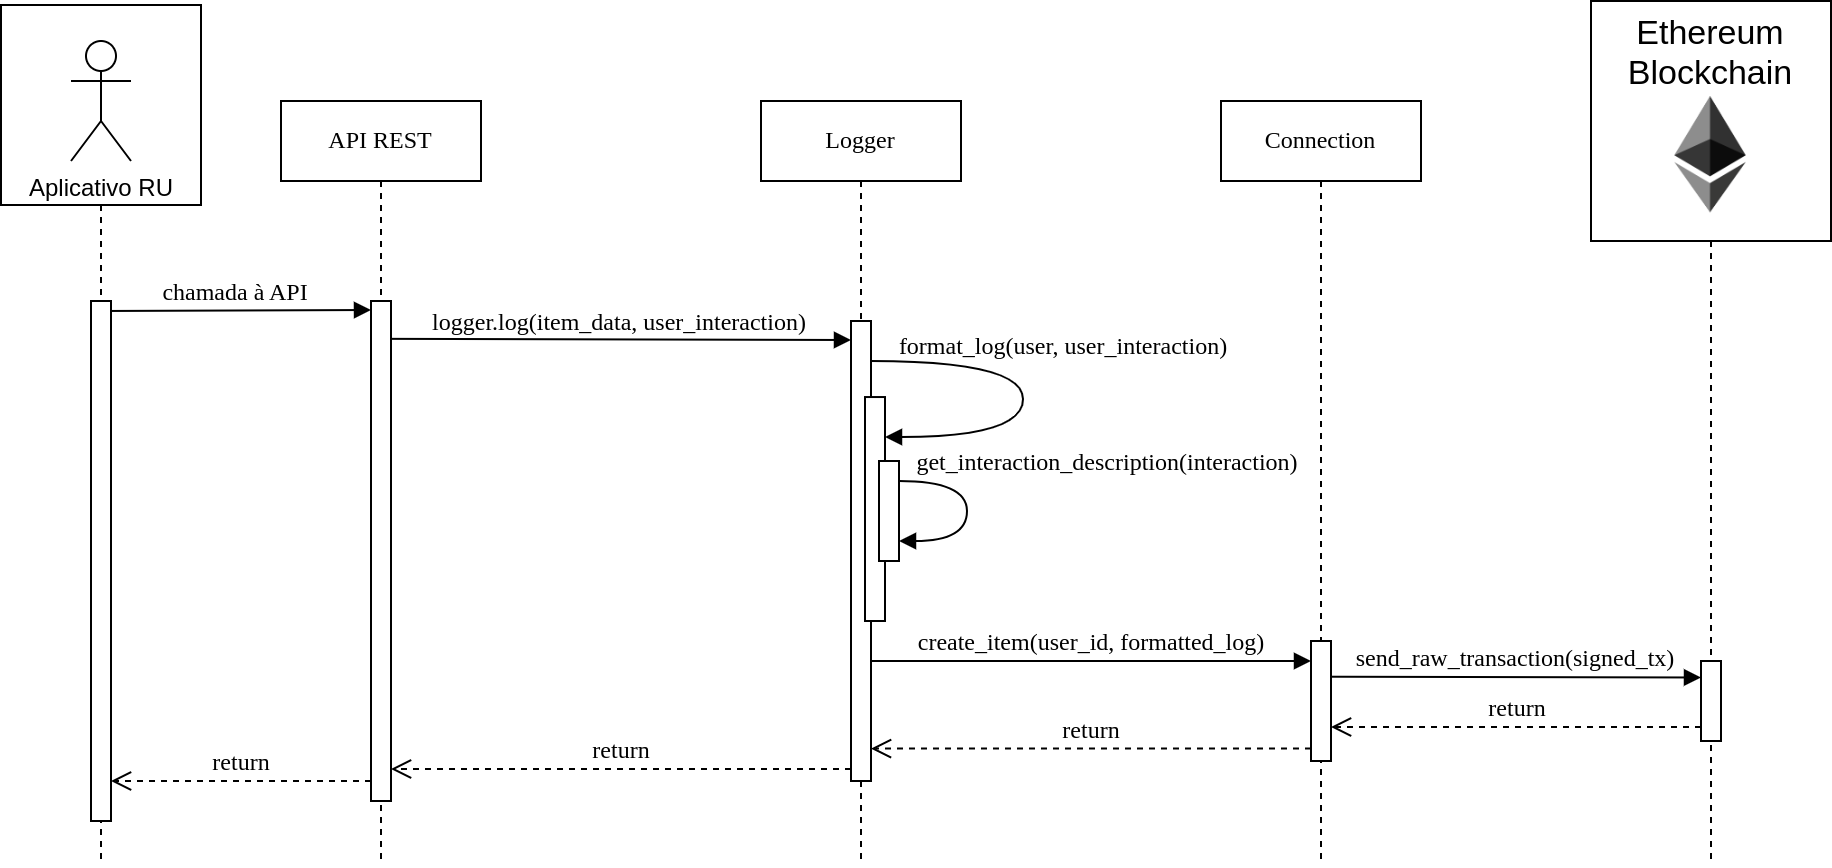
\includegraphics[width=1\textwidth]{img/Cap3/diagramas/Diagrama de Sequência.drawio.png}
    \caption{Diagrama de Sequência da aplicação}
    \label{fig:diagrama_sequencia}
\end{figure}
Com o Diagrama de Sequência conseguimos obter uma visão de como o sistema age para alcançar determinado fim. Nele existem os participantes, as partes do sistema que interagem umas com as outras durante uma sequência \cite{Miles2006-fo}. Dispostos de maneira horizontal entre si, os participantes possuem uma reta vertical em baixo, chamada de linha de vida, ilustrando o seu estado em um determinado instante de tempo.

O diagrama da Figura \ref{fig:diagrama_sequencia} demonstra o encadeamento lógico da troca de mensagens entre os diferentes participantes do sistema, dando ênfase à ordem temporal em que as mensagens foram trocadas. Similar ao Diagrama de Casos de Uso, o Diagrama de Sequência também define atores, entidades que, juntamente com os objetos do sistema, formam os participantes que participam de toda a interação. A mensagem inicial parte do aplicativo Carteira Digital do Restaurante Universitário da UEA, realizando uma chamada à API REST, que então utiliza objetos instanciados do sistema para realizar a lógica de negócio, por fim, culminando na comunicação com a Blockchain Ethereum.

\newpage
\begin{figure}
    \centering
    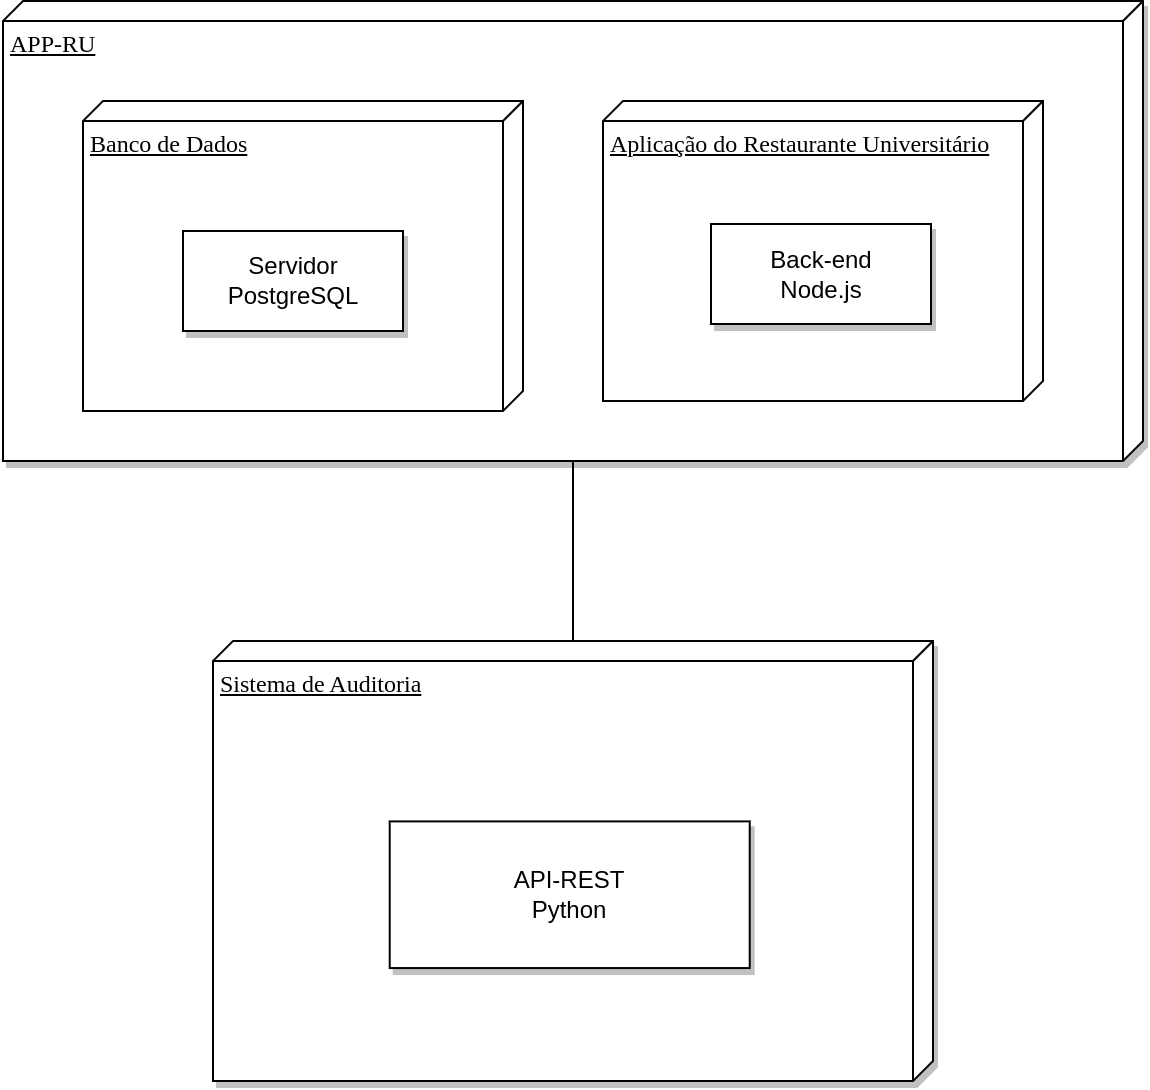
\includegraphics[width=0.8\textwidth]{img/Cap3/diagramas/Diagrama de Implantação.drawio.png}
    \caption{Diagrama de Implantação da aplicação}
    \label{fig:diagrama_implantacao}
\end{figure}
\subsection{Diagrama de Implantação}
O Diagrama de Implantação mostra as necessidades do sistema quanto ao \emph{hardware} a ser utilizado. Em termos práticos, este diagrama elenca os diferentes nós presentes no sistema e suas características, que, segundo \cite{Guedes2018}, são características físicas como servidores, estações, topologias e protocolos de comunicação, ou seja, todo o aparato físico sobre o qual o sistema deverá ser executado.

Componentes de \emph{software} executados, chamados de artefatos, também aparecem no diagrama, como demonstrado na Figura \ref{fig:diagrama_implantacao}. As interações entre os nós a partir de sua conectividade é uma importante informação expressa pelo diagrama de implantação.


\newpage
\subsection{Diagrama de Classes}
\begin{figure}
    \centering
    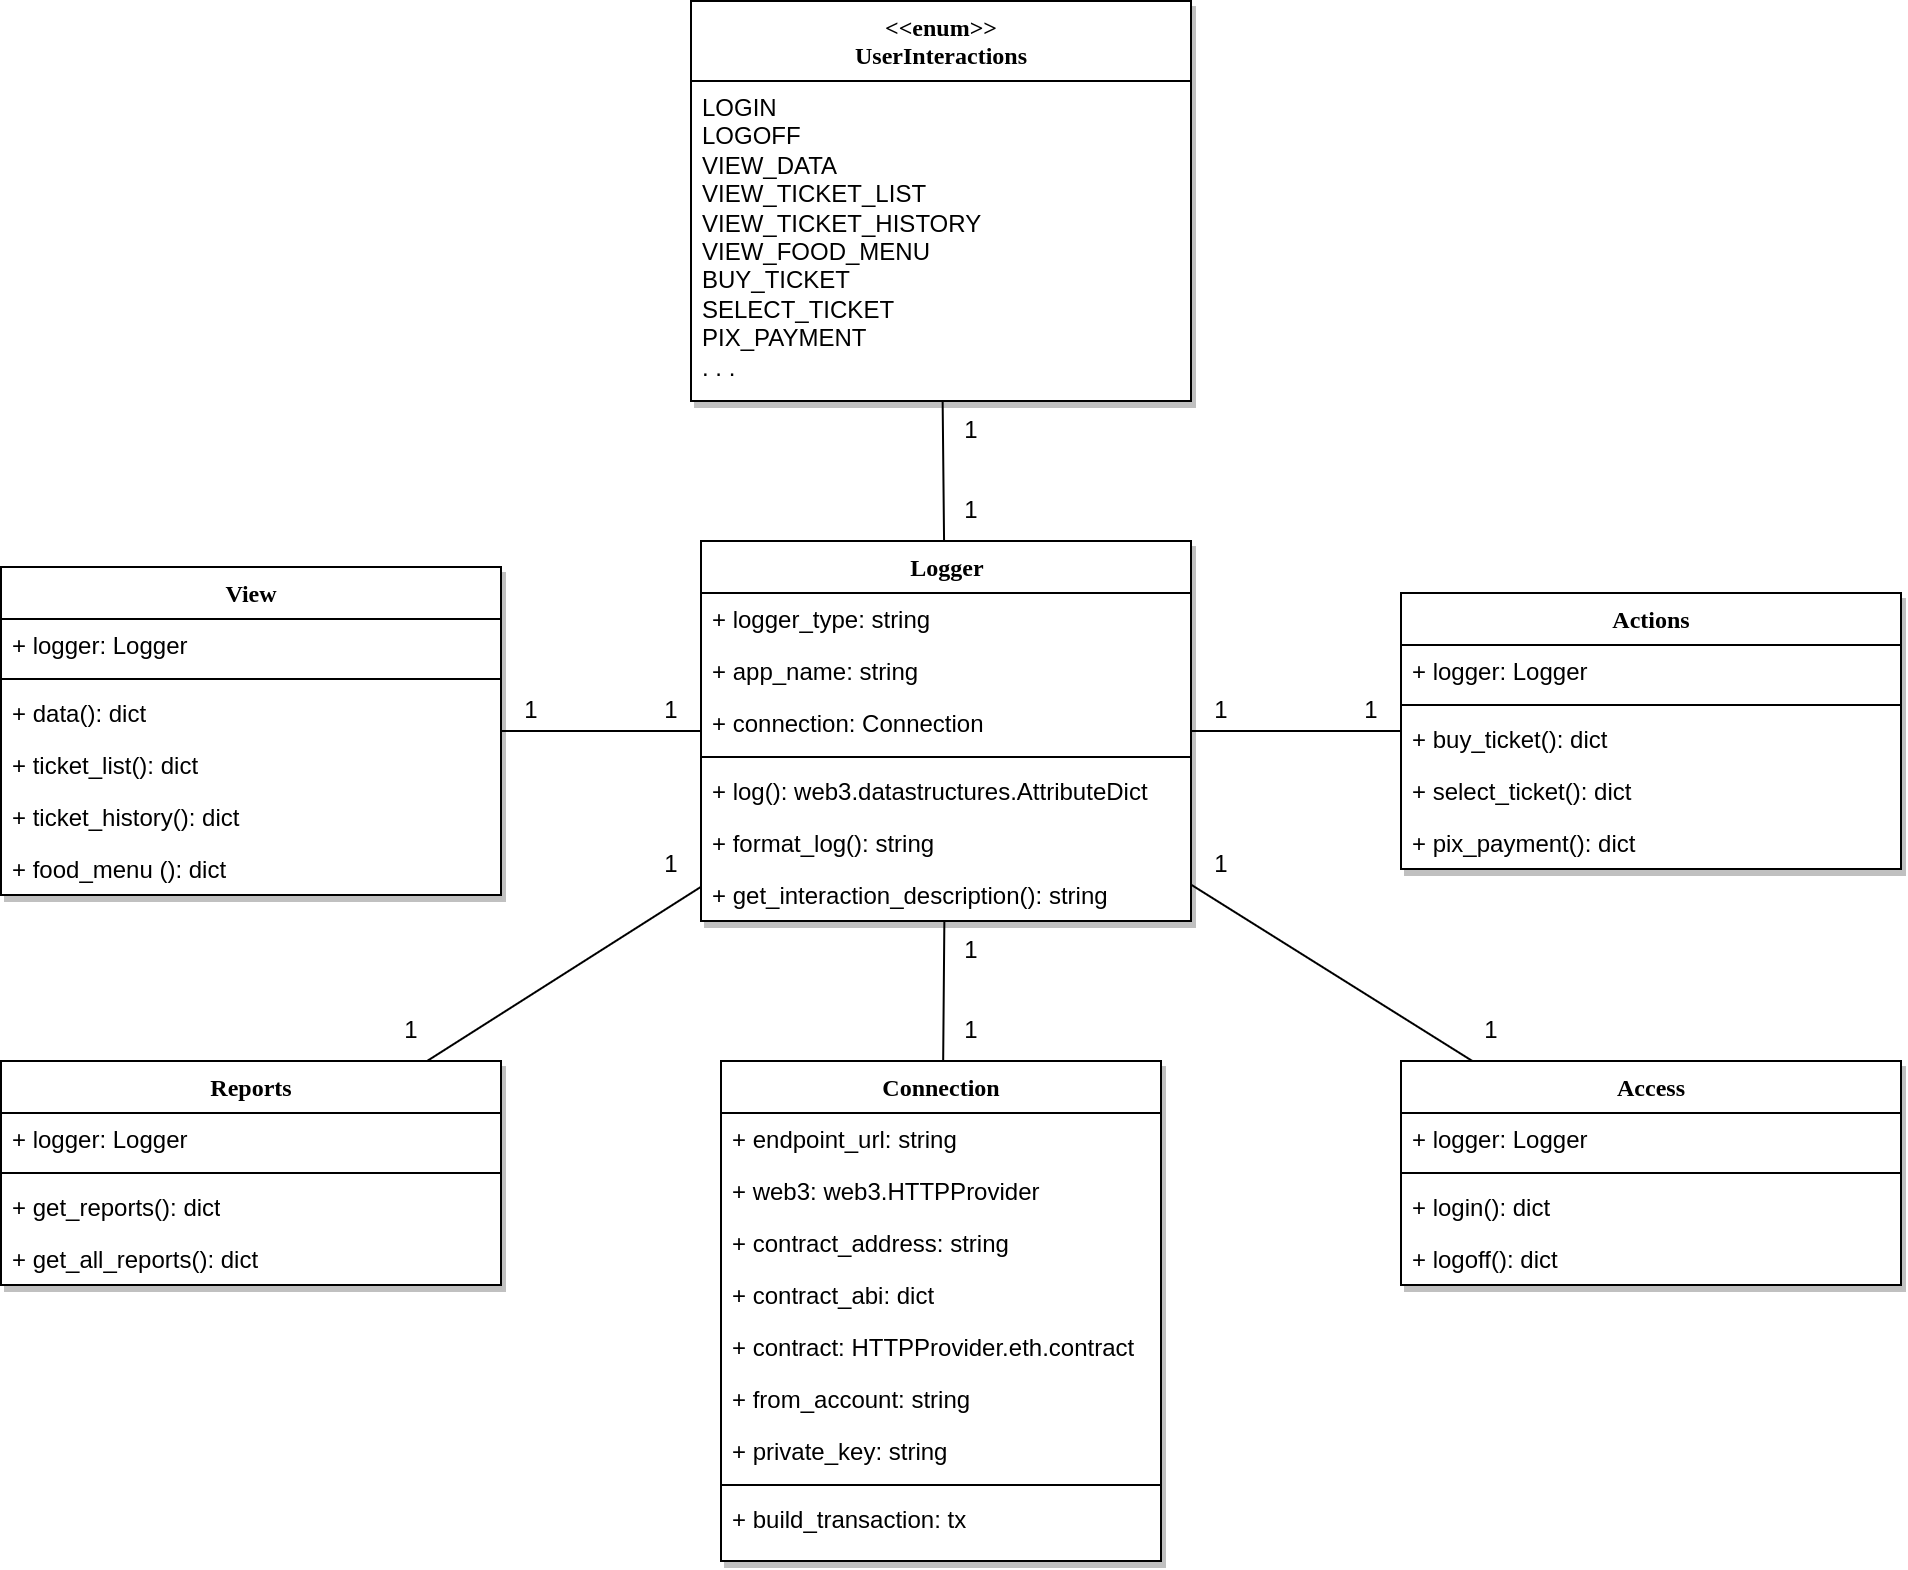
\includegraphics[width=1\textwidth]{img/Cap3/diagramas/Diagrama de Classes.png}
    \caption{Diagrama de Classes da aplicação}
    \label{fig:diagrama_classes}
\end{figure}

Um Diagrama de Classes define as classes presentes no sistema e seus relacionamentos. Uma classe é a base para um objeto que será instanciado e utilizado na aplicação. Cada classe possui atributos e métodos próprios, além da possibilidade de realizar associações entre si.

Quatro das classes retratadas no diagrama da Figura \ref{fig:diagrama_classes} se referem aos diferentes tipos de interações que são interpretadas pela API:
\begin{itemize}
    \item A classe Access implementa métodos de acesso ao sistema, como \emph{login} e \emph{logoff}
    \item A classe Actions implementa métodos de ações gerais realizadas pelo usuário, como a compra de um ticket
    \item A classe View emprega funcionalidades de visualização de dados em geral
    \item A classe Reports dá suporte à obtenção de dados salvos e à geração de relatórios
\end{itemize}

O centro de toda a aplicação jaz na classe Logger. Esta classe tem por objetivo criar as mensagens de \emph{logs} que serão persistidas na rede Blockchain. Para isso, utiliza uma instância da classe Connection, responsável por realizar a conexão com a plataforma Ethereum e realizar operações diversas. A classe Logger também faz uso de uma classe de suporte chamada UserIteractions, enumerando os tipos de interações possíveis dentro do contexto da aplicação.


\section{Implementação da solução}
O sistema de auditoria tem como base uma API REST implementada na linguagem de programação Python, sendo responsável por captar requisições de um cliente e as processar. A depender do tipo de requisição recebida, o sistema apresenta diferentes tipos de comportamentos e estrutura suas respostas de maneira análoga. \emph{Endpoints}, ou pontos de extremidade de uma API, são os locais onde são recebidas as chamadas ao sistema. Estes \emph{endpoints} são chamados por meio de \emph{URIs} específicas, que por sua vez são mapeadas diretamente a funções dentro da aplicação Python.

A API REST, devido à sua conexão com a rede Ethereum, provê dois tipos diferentes de chamadas: funções que alteram o estado e funções que visualizam o estado. Devido à natureza de uma Blockchain, transações realizadas na rede necessitam de um pagamento para serem concretizadas, ao tempo que operações de leitura da rede não possuem custo operacionais. A escrita de mensagens de \emph{log} é um ato de persistência de informação na rede, possuindo assim um certo custo inerente; a visualização destes \emph{logs}, por sua vez, é um ato não dispendioso.

A implementação da API REST deu-se a partir de uma imagem Docker da linguagem de programação Python. Desta forma, todas as dependências da aplicação são isoladas de todo o resto do sistema, reduzindo drasticamente problemas de conflito de versões e aumentando a portabilidade da solução.

\subsection{Conexão com a plataforma Ethereum}
\begin{figure}
    \includegraphics[width=0.4\textwidth]{img/Cap3/blockchain/Conexão 1.png}
    \centering
    \includegraphics[width=0.4\textwidth]{img/Cap3/blockchain/Conexão 2.png}
    \caption{Demonstração da implantação de um contrato inteligente via MetaMask}
    \label{fig:smart_contract}
\end{figure}
Para manipular dados na Blockchain é necessário ter em posse uma carteira de criptomoedas, possibilitando assim a realização de transações na rede. Como existem várias maneiras de se criar uma carteira, optou-se pelo uso do \emph{software} MetaMask para sua criação e manutenção. O MetaMask é uma extensão de navegador que permite que usuários armazenem e gerenciem contas, além de possibilitar a comunicação com aplicações descentralizadas. A Figura \ref{fig:smart_contract} mostra uma carteira configurada com diferentes contas.

A partir da carteira criada pelo MetaMask, criaram-se contas capazes de serem usadas na rede Ethereum e suas \emph{testnets}. Cada conta é composta em sua essência por um par de chaves: a chave pública e a chave privada. A chave pública é derivada da chave privada e pode ser compartilhada e usada por qualquer um para verificar assinaturas digitais feitas pela chave privada, que por sua vez é utilizada para comprovar posse de contas ou contratos da Blockchain. 

\begin{figure}
\centering
    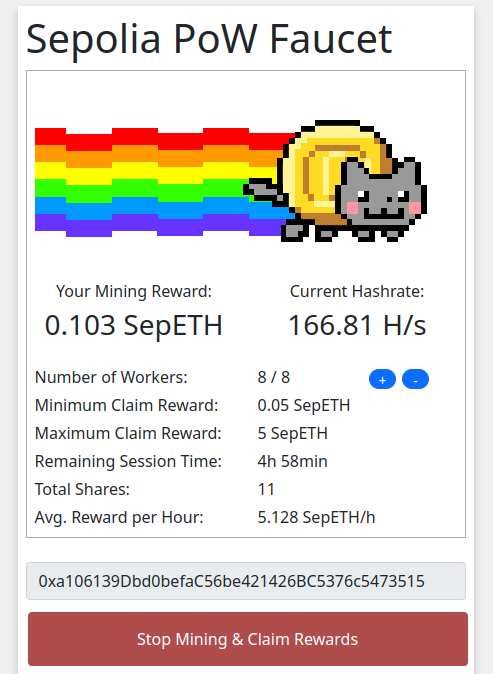
\includegraphics[width=0.5\textwidth]{img/Cap3/blockchain/faucet.png}
    \caption{Obtenção de criptomoedas de teste para a \emph{testnet} Sepolia}
    \label{fig:faucet}
\end{figure}

As quantias de criptomoedas das contas criadas são provenientes de  \emph{faucets}. Cada \emph{faucet} costuma ser especializada em uma \emph{testnet} específica. Particularmente, a principal \emph{faucet} utilizada foi a Sepolia PoW Faucet \cite{pow_faucet}, hospedada em \emph{websites} que se dispõem a depositar Ether à um endereço da Blockchain em troca de tarefas de mineração concretizadas pelo computador do usuário. A quantidade de criptomoeda recebida é proporcional ao tempo e esforço computacional realizado. A Figura \ref{fig:faucet} demonstra um processo de mineração em andamento pelo \emph{website}, provendo uma remuneração com base na quantidade de cálculos executados pelo computador.

Para salvar as mensagens de \emph{log} foi implementado um contrato inteligente na linguagem de programação Solidity; desta forma, é possível executar chamadas ao contrato após o seu processo de implantação na rede (\emph{deploy}). O desenvolvimento do contrato se deu por meio da plataforma Remix IDE, que provê um ambiente de desenvolvimento próprio para a confecção de contratos inteligentes. Após sua escrita, o contrato é compilado para então, finalmente, ser lançado na rede Ethereum. 

O contrato inteligente implementa uma estrutura de dados chamada \emph{mapping}, que mapeia uma determinada entrada a uma única saída, similar a uma tabela de dispersão (também conhecida como \emph{hash}). Devido a natureza da Blockchain, operações de persistência na rede exigem certa quantidade de criptomoeda para serem executadas; para isso, realiza-se a criação de uma transação a partir dos dados recebidos, que é assinada com a chave privada da conta utilizada pela API. Isso garante o envio da transação de forma única e inequívoca por parte do sistema. O dado utilizado na estrutura de mapeamento é o id, a identificação única do usuário no contexto do sistema, que aponta para uma estrutura de dados do tipo lista, responsável por guardar as mensagens de log recebidas pela aplicação. Operações de visualização de dados, por sua vez, não possuem custo de execução e podem ser executadas livremente, retornando para a API REST todos os dados salvos. Como o contrato inteligente é um endereço público na Blockchain, uma camada de segurança, em tempo de execução do contrato, foi empregada: apenas a conta que é dona do contrato, ou seja, a conta que realizou a implantação do contrato na rede, é capaz de chamar os métodos do contrato.

\begin{figure}
    \centering
    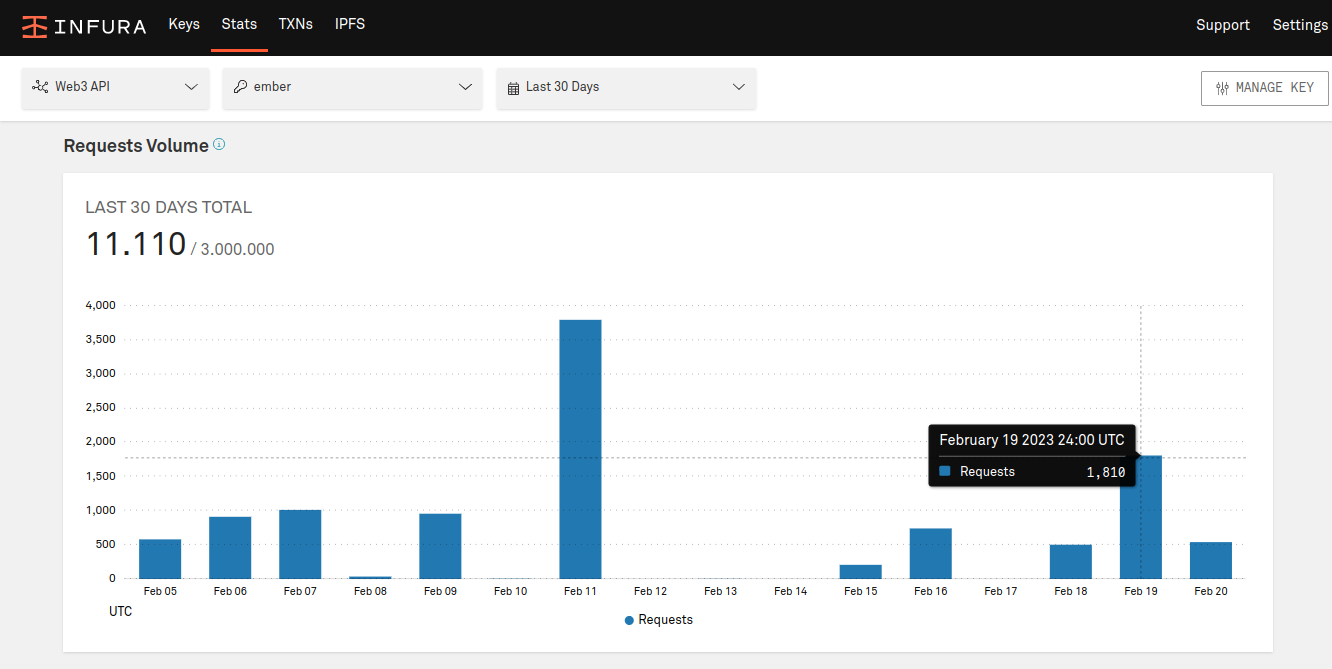
\includegraphics[width=1\textwidth]{img/Cap3/blockchain/Infura estatisticas.png}
    \caption{Gráfico de requisições realizadas fornecido pelo provedor Infura}
    \label{fig:infura_estatisticas}
\end{figure}
Para interagir com o contrato inteligente, a API REST necessita se comunicar com a Blockchain. Esta necessidade é sanada com o uso de um provedor Infura. Infura é o nome de um serviço de estrutura de nó (\emph{node infrastructure}) que provê acesso confiável para a rede Ethereum. A partir de sua API, o Infura permite acesso instantâneo à rede por meio do protocolo HTTPS e de WebSockets. A biblioteca Web3.py faz uso da url do provedor, que contém a chave de API necessária para concretizar a comunicação.

A partir da conexão com o provedor Infura, é possível fazer chamadas ao contrato inteligente implantado na Blockchain. A biblioteca Web3.py é capaz de fazer chamadas a métodos do contrato após a sua implantação na rede com o uso de seu endereço único. Para isso, são passados os parâmetros correspondentes necessários para a chamada de uma função do contrato. A plataforma disponibiliza um \emph{dashboard}, tal como na Figura \ref{fig:infura_estatisticas}, para a visualização de estatísticas de uso do provedor, como o número de requisições efetuadas em determinado período de tempo.

\begin{figure}
\centering
    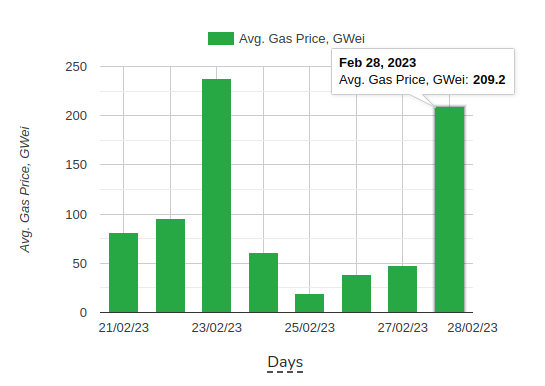
\includegraphics[width=0.8\textwidth]{img/Cap3/blockchain/goerli gas.png}
    \caption{Súbita variação do preço de \emph{gas} na \emph{testnet} Goerli \cite{Bitquery}}
    \label{fig:goerli_gas}
\end{figure}
A escolha da \emph{testnet} utilizada baseou-se na alternativa mais bem difundida, que é a rede Goerli. No entanto, altas flutuações no tráfego da rede a tornaram uma alternativa inviável devido ao súbito aumento do preço do \emph{gas}, como expresso no gráfico da Figura \ref{fig:goerli_gas}. Segundo Marius van der Wijden, desenvolvedor da plataforma Ethereum, este encarecimento no preço das transações da rede é um comportamento esperado com todas as \emph{testnets} \cite{kelly_2023}. Segundo o desenvolvedor, o plano é fazer uma lenta migração de usuários da rede Goerli para a rede Sepolia. A rede Sepolia foi criada com o intuito de ajudar desenvolvedores testarem suas aplicações descentralizadas em um ambiente mais realista e que mais se assemelha à \emph{mainnet} Ethereum \cite{porcelli_2023}. Portanto, optou-se por migrar o contrato inteligente implementado para a \emph{testnet} Sepolia, sem grandes perdas. 


\subsection{Mensagens de \emph{log}}
O sistema de auditoria para o aplicativo Carteira Digital do Restaurante Universitário da UEA tem por objetivo registrar, de forma permanente, as interações realizadas pelos usuários do aplicativo. Atos como entrar no aplicativo, a compra de um ticket de alimentação e a visualização do cardápio são registradas de maneira segura na rede Blockchain, impedindo assim quaisquer ações com o intuito de adulteração de dados. Os registros, ou \emph{logs}, possuem a seguinte estrutura:

\begin{table}[H]
    \centering
    \begin{tabular}{| p{14cm} |}
        \hline
         2023-01-01 08:00:00 APP\_RU:view | 'nome' [id] viewed the food menu \\
        \hline
    \end{tabular}
    \label{tab:estrutura_log}
\end{table}
De forma que cada parte da mensagem possui um significado:
\begin{table}[H]
    \centering
    \begin{tabular}{ | p{4cm} | p{10cm} |}
        \hline
        \textbf{Mensagem} & \textbf{Descrição}\\
        \hline
        
        2023-01-01 & Data da interação a ser registrada, no formato YYYY-MM-DD \\
        \hline

        08:00:00 & Hora da interação a ser registrada, no fuso horário GMT-4 (America/Manaus) \\
        \hline

        APP\_RU:view & Nome da aplicação executada seguida do módulo do sistema \\
        \hline

        | & Caractere delimitador que isola dados da mensagem \\
        \hline

        'nome' {[}id{]} & Nome de usuário no qual ficará registrada a ação efetuada (opcional), dentro de aspas simples; id do usuário, dentro de colchetes \\
        \hline      

        viewed the food menu & Ação efetuada pelo usuário \\
        \hline      
    \end{tabular}
    \caption{Estrutura da mensagem de \emph{log}}
    \label{tab:estrutura_log}
\end{table}

Cada interação configura o registro de um \emph{log} informacional na Blockchain. A estrutura de uma mensagem de \emph{log} é fixa e padronizada com o intuito de facilitar auditorias do sistema, sendo composta por um cabeçalho e um corpo. No cabeçalho são definidos metadados para caracterizar a mensagem de \emph{log} a ser armazenada, sendo utilizadas data, hora e a fonte, referenciando qual parte do sistema foi recebeu uma chamada e foi executada. O corpo da mensagem, por sua vez, carrega consigo a informação necessária para identificar a entidade e sua ação direta no sistema, garantindo assim irretratabilidade ou não repúdio. Desta forma, uma vez executada por um usuário, uma ação não pode ser negada e nem desfeita e sempre apontará para o indivíduo que a realizou.

Para facilitar a visualização, optou-se por separar o cabeçalho e corpo da mensagem por um delimitador, para isso foi utilizado o caractere \emph{pipe} (|), ou barra vertical, com o intuito de alinhar as mensagens em relação ao caractere.

\subsection{Trilhas de auditoria}
\begin{figure}
    \centering
    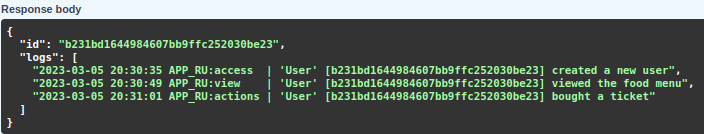
\includegraphics[width=1\textwidth]{img/Cap3/Trilha de auditoria.png}
    \caption{Exemplo de trilha de auditoria fornecida pela API REST}
    \label{fig:trilha_auditoria}
\end{figure}

O conjunto de ações efetuadas pelo usuário, no contexto do sistema, é registrado, compondo assim uma trilha de auditoria acessível a qualquer momento. A trilha de auditoria, sendo um elemento fundamental na responsabilização das partes, deve ser íntegra e corresponder com a realidade, o que é alcançado com o uso da rede Ethereum.

Após o usuário realizar uma ação, uma chamada é disparada à API REST. Num primeiro momento, os dados são capturados e então passam por um processo chamado de serialização, no qual são traduzidos para uma estrutura em que a linguagem de programação consiga entender. Em seguida, as informações são utilizados pela lógica de negócio. 

Para salvar a mensagem correta no \emph{log}, a classe responsável pela sua construção se relaciona com uma classe de suporte chamada UserInteraction, que implementa um Enum, um tipo de dados abstrato utilizado para enumerar um conjunto finito de opções, que neste caso são os tipos de interações possíveis com o sistema. Para cada tipo de Enum presente nesta classe está configurada uma mensagem. A Figura \ref{fig:trilha_auditoria} ilustra diferentes mensagens presentes em uma trilha de auditoria de um usuário.


\section{Integração com o aplicativo Carteira Digital do Restaurante Universitário da UEA}
No processo de desenvolvimento de um sistema, a integração de sistemas é um estágio em que componentes são colocados juntos para a criação de um novo sistema \cite{Sommerville2011}. Para realizar a integração do \emph{back-end} do aplicativo do Restaurante Universitário da UEA, foi necessário, inicialmente, executar o sistema em um ambiente próprio. Com isso, uma análise geral da construção do projeto fez-se necessário, desde a instalação de dependências até um estudo preliminar do código-fonte.

A tecnologia utilizada para o \emph{back-end} da aplicação do RU é o Node.js, um ambiente (\emph{runtime environment}) para servidores orientados a eventos que faz uso da linguagem de programação Javascript para processar requisições de clientes. Junto ao Node.js, o projeto emprega o \emph{software} PostgreSQL para atuar como SGDB (Sistema de Gerenciamento de Banco de Dados) da aplicação, responsável por criar, manter e manipular bancos de dados. Para dar suporte à tarefas de banco de dados, o sistema recorre ao Prisma, um ORM (\emph{Object-Relational Mapper}) ou mapeador objeto-relacional com o intuito de mitigar riscos envolvidos na livre escrita de consultas de dados na aplicação, como ataques de injeção SQL e agilizar o desenvolvimento da aplicação.

\begin{figure}
    \centering
    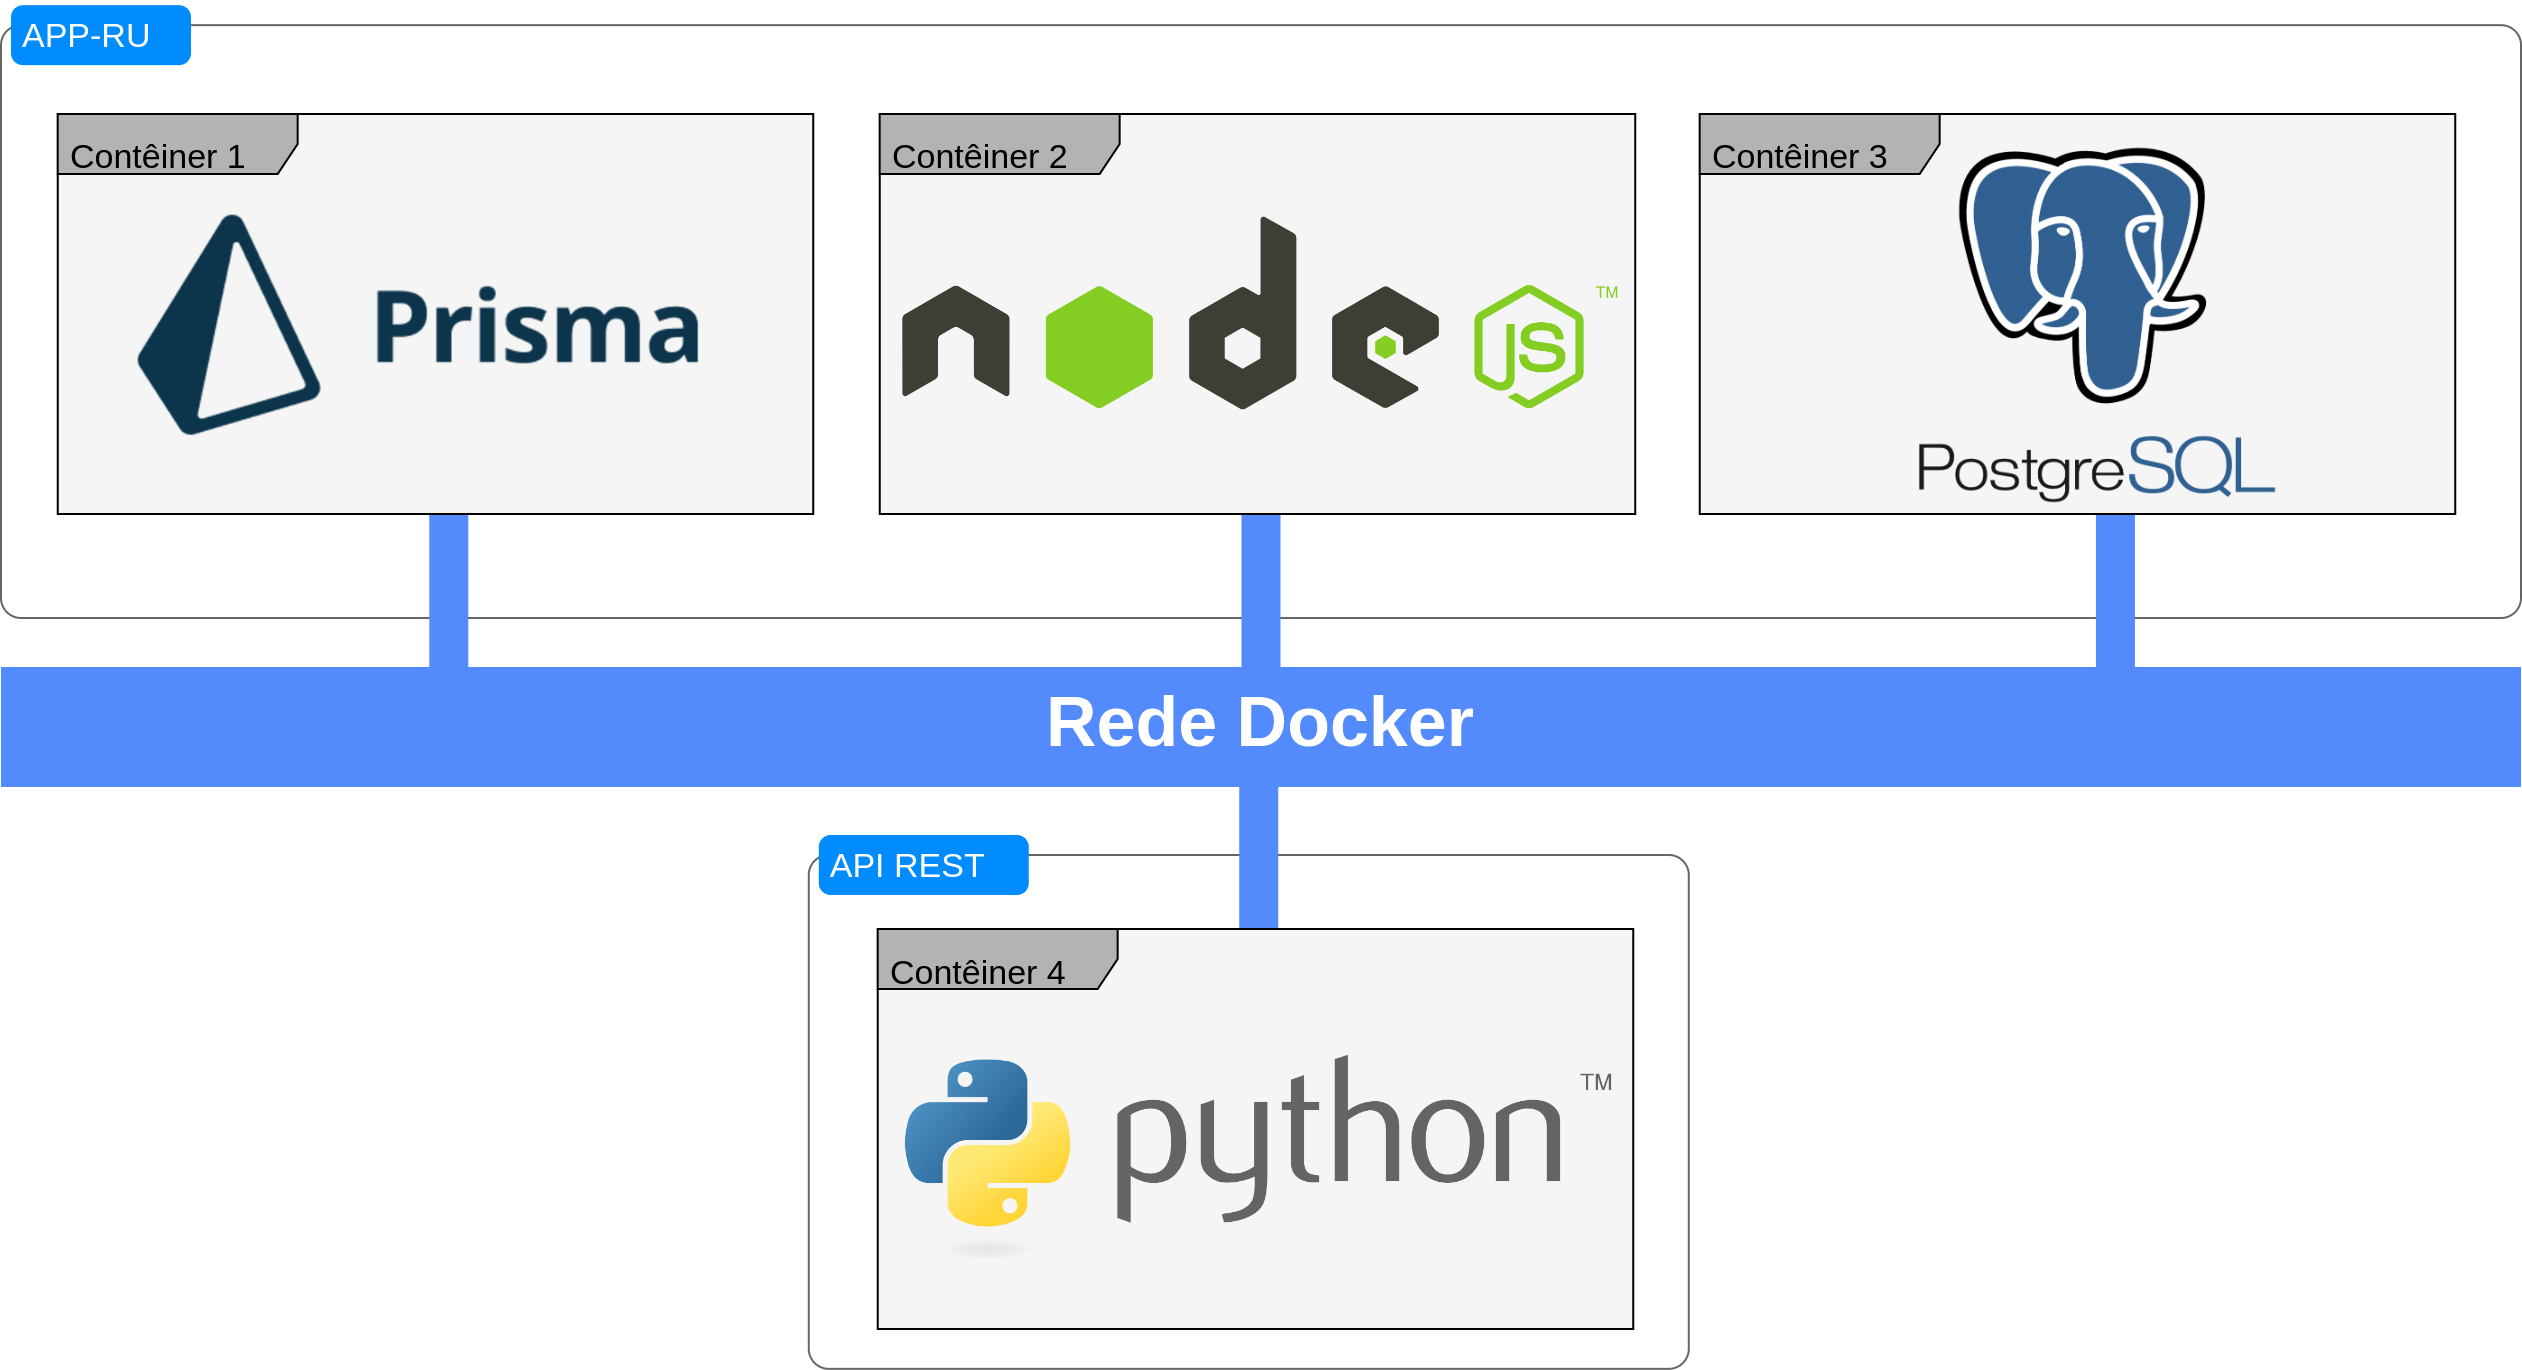
\includegraphics[width=1\textwidth]{img/Cap3/Rede Docker.png}
    \caption{Rede formada pelos diferentes contêineres com o docker-compose}
    \label{fig:rede_docker}
\end{figure}


Todas as tecnologias descritas anteriormente integram-se a partir do Docker, que é responsável por executar um contêiner por serviço e gerenciar as comunicações entre cada um deles. O diagrama da Figura \ref{fig:rede_docker} ilustra a conexão entre os diferentes contêineres. Para isso, utiliza-se a ferramenta \emph{docker-compose}, fazendo com que cada um dos contêineres passem a se enxergar e comuniquem-se entre si de forma totalmente transparente, como em uma rede. O \emph{docker-compose} é uma ferramenta que define os componentes de uma aplicação (como contêineres, volumes e configurações) em um único arquivo \cite{Raj2015-ju}, garantindo assim ao desenvolvedor a possibilidade de executar o sistema mais facilmente, simplificando instalações e futuras implantações do \emph{software}.

Parte do esforço de integração entre diferentes sistemas se dá, num primeiro momento, na configuração do ambiente de ambas as partes a serem integradas. Segundo \cite{Sommerville2011}, em integrações entre diferentes sistemas a fim de se criar um único, uma fração significativa do desenvolvimento preocupa-se com a configuração do sistema e não com o desenvolvimento de código original. 

Adaptações necessárias ao código fonte do APP-RU também foram necessárias, a fim de que passe a ser registrada cada ação tomada por um usuário deste sistema. No caso de um utilizador do sistema criar um novo usuário para si, visualizar o cardápio do restaurante e em seguida comprar um ticket, cada uma destas ações é registrada de forma individual, garantindo rastreabilidade nos passos seguidos por este utilizador da aplicação. Para isso, incluiu-se no código-fonte chamadas à API REST, conforme o tipo de requisição processada pelo \emph{back-end} do APP-RU.


\section{Testes na aplicação}
Testes de \emph{software} foram implementados para garantir qualidade à aplicação desenvolvida, além de promover a redução de risco de falhas, devido à descoberta de possíveis erros de execução. A abordagem escolhida foi a utilização de testes de caixa-preta para testar os \emph{endpoints} da API REST. Os tipos de testes empregados são testes de unidade e testes de integração.

Os testes de unidade são utilizados para testar unidades individuais para o sistema, que para \cite{Pressman2021-jj} são os componentes, com a finalidade de garantir que sua função esteja sendo desempenhada de maneira correta. Testes de integração, por sua vez, visam testar a conjunção de diferentes componentes que interagem entre si \cite{Pressman2021-jj}. É um tipo de teste necessário pois mesmo que dois componentes distintos funcionem normalmente de forma isolada, existe a chance de que haja algum tipo de erro na ponte que faz ligação com ambos, ou seja, na interface.

Após ser realizada uma transação na Blockchain, a rede retorna um objeto contendo metadados desta transação, que são utilizados como parâmetro principal do teste realizado. Um atributo deste objeto é o atributo \emph{status}, que pode possuir ou o valor 1, denotando sucesso na transação, ou o valor 0, denotando uma falha no processo. Esta resposta recebida pela Blockchain após ser realizada uma transação é o que fundamenta o teste. Erros em tempo de execução também são levados em conta: se houver qualquer tipo de exceção não tratada dentro do código, o teste falha, apontando o erro e a linha onde ele ocorreu.

\subsection{Testes de unidade e integração}
\begin{figure}
    \centering
    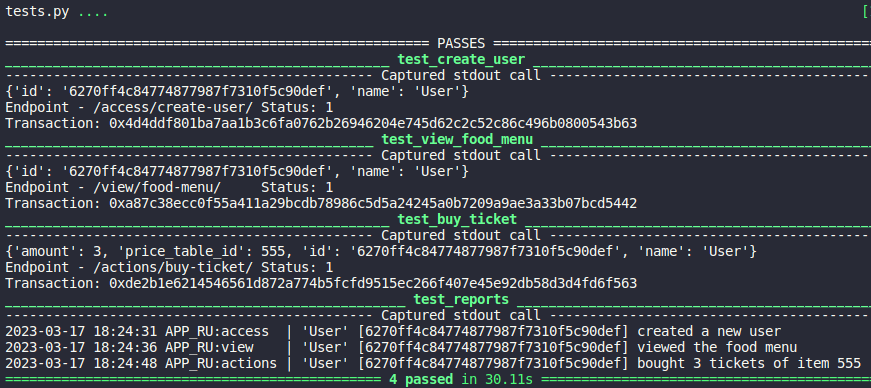
\includegraphics[width=1\textwidth]{img/Cap3/teste de unidade.png}
    \caption{Teste de unidade realizado com id gerado de forma aleatória}
    \label{fig:teste_unidade}
\end{figure}

Para realizar os testes de unidade e de integração foi utilizada a ferramenta pytest. Ela executa um código composto por diversas funções prefixadas com a palavra "\emph{test}", cada uma referenciando um caso de teste diferente, observando a aparição de possíveis erros no código em tempo de execução. Caso não haja nenhum tipo de erro, é dito que a função executada foi bem sucedida e passou no teste.

Devido à grande quantidade de \emph{endpoints} diferentes, optou-se por testar um \emph{endpoint} para cada módulo do sistema devido ao fato de cada módulo implementar uma classe única. Desta forma, foram escolhidos os \emph{endpoints} de criação de usuário, de visualização do cardápio e de compra de ticket.

A biblioteca pytest executa funções encarregadas de mandar requisições para a API REST. A depender do \emph{endpoint}, diferentes argumentos são passados para concretizar a requisição e estruturar a mensagem de \emph{log}. Os testes de unidade são realizados por meio de chamadas diretas à API REST, visando testar o funcionamento dos módulos. Os testes de integração, por sua vez, são feitos com chamadas à API REST realizadas pelo \emph{back-end} da aplicação do Restaurante Universitário. Ambos os testes possuem a mesma saída, que é expressa na Figura \ref{fig:teste_unidade}.



\chapter{Conclusão}
Este capítulo tem por objetivo expor os resultados alcançados após o desenvolvimento da solução, além de comentar a sua eficácia para a resolução do problema proposto. Ideias de trabalhos futuros também são sugeridas, a fim de incrementar as funcionalidades do sistema desenvolvido e torná-lo mais eficiente.

\section{Resultados}
O sistema desenvolvido foi uma API REST para dar suporte a processos de auditoria para o aplicativo Carteira Digital do Restaurante Universitário da UEA. Para isto, foi feita uma integração com o \emph{back-end} do aplicativo do Restaurante Universitário, possibilitando ao sistema fazer chamadas à API para salvar mensagens de \emph{log}, que são confeccionadas com base no usuário que está se comunicando com o sistema e a interação efetuada por ele.

\begin{figure}
    \centering
    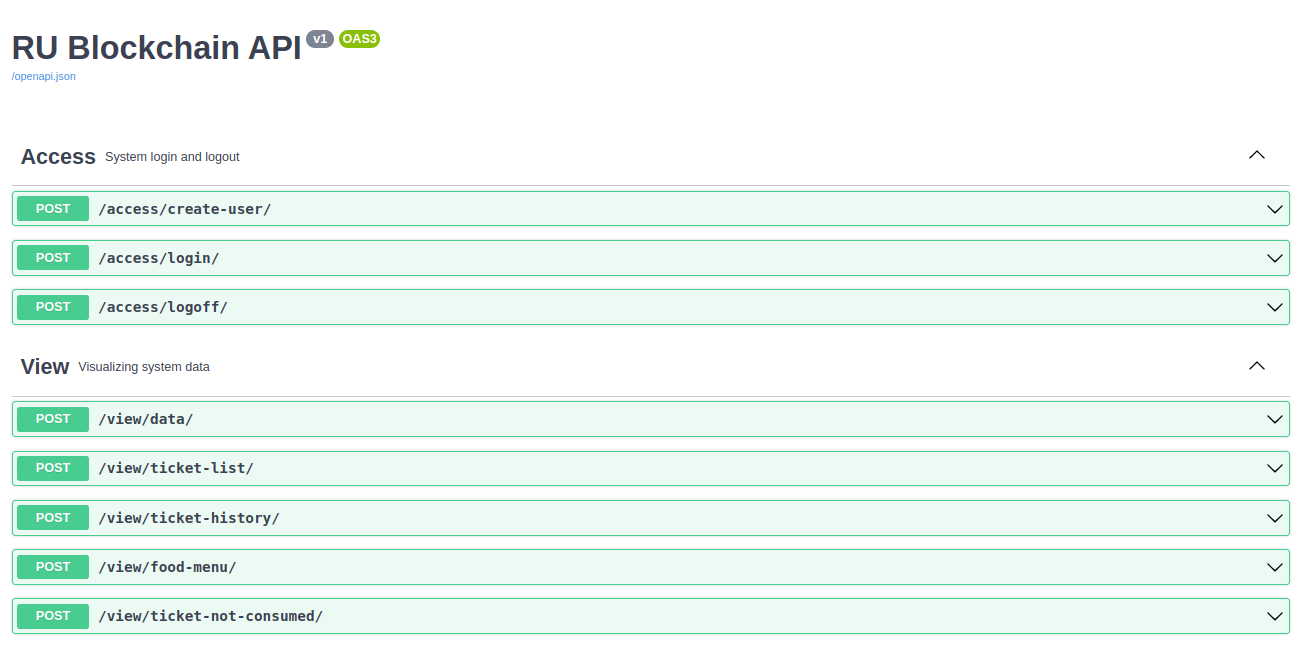
\includegraphics[width=1\textwidth]{img/Cap4/Swagger.png}
    \caption{Parte da página \emph{web} gerada pela documentação OpenAPI}
    \label{fig:openapi}
\end{figure}

A API REST segue a especificação OpenAPI 3.0 (também conhecido como Swagger, em versões anteriores), que define uma interface uniforme, independente de linguagem de programação, para descrever APIs e tornar capaz o seu entendimento tanto por humanos quanto por computadores \cite{openapi_specification}. Com isto, é possível acessar uma página \emph{web} contendo a definição da API REST criada, listando todos os \emph{endpoints} disponíveis, separados por módulo. A Figura \ref{fig:openapi} demonstra parte da documentação gerada pela aplicação. 

Cada um dos \emph{endpoints} da aplicação recebe uma requisição quando o usuário executa a ação relacionada a ele. Se uma pessoa cria um novo usuário, por exemplo, o \emph{back-end} da aplicação do Restaurante Universitário dispara uma requisição para o \emph{endpoint} \emph{/access/create-user/} da Figura \ref{fig:openapi}, enviando os parâmetros necessários para figurar o registro de uma mensagem de \emph{log} na Blockchain.

\begin{figure}
    \centering
    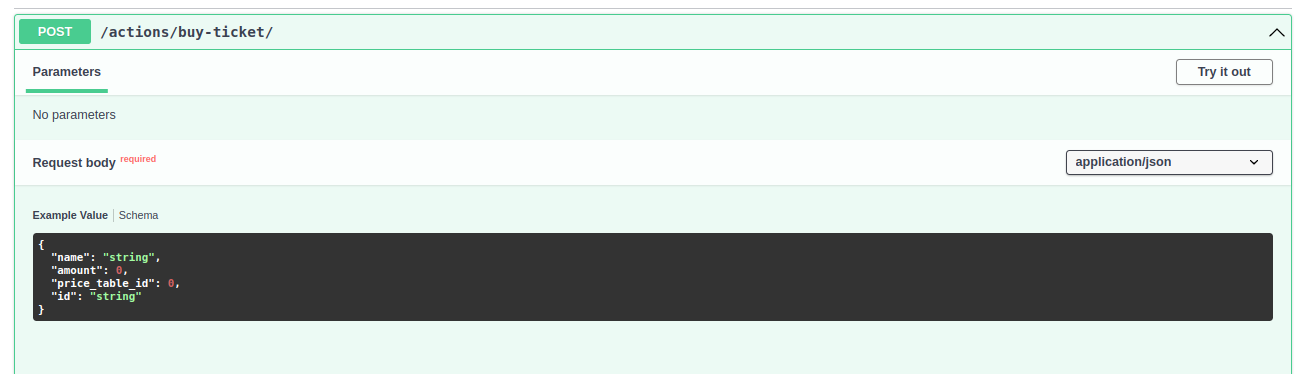
\includegraphics[width=1\textwidth]{img/Cap4/endpoint.png}
    \caption{\emph{Endpoint} para a compra de tickets e seus parâmetros}
    \label{fig:endpoint}
\end{figure}

Os parâmetros utilizados numa requisição podem variar de \emph{endpoint} para \emph{endpoint}. Em geral, todos recebem um valor referente à identificação única do usuário dentro do sistema e, opcionalmente, um valor referente ao nome do usuário. A Figura \ref{fig:endpoint} demonstra os parâmetros necessários para uma requisição de compra de ticket, sendo necessário informar a quantidade de tickets comprados e o id do item comprado a fim de que seja realizado o registro da mensagem.

\begin{figure}
    \centering
    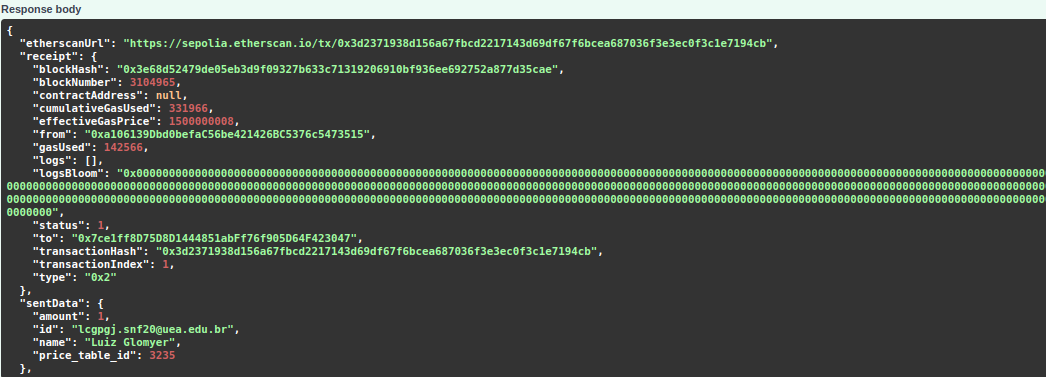
\includegraphics[width=1\textwidth]{img/Cap4/resposta.png}
    \caption{Estrutura da resposta da API após uma requisição}
    \label{fig:resposta}
\end{figure}

Após uma requisição, a mensagem é armazenada na Blockchain, retornando os metadados da transação efetuada, conforme mostra a Figura \ref{fig:resposta}. Informações como o bloco da transação e o seu hash são úteis para confirmar que a transação realmente foi realizada na rede. A partir de seu hash podemos observar mais a fundo as características da transação efetuada com o uso do Etherscan, um \emph{website} que agrega transações feitas na rede. O Etherscan (Figura \ref{fig:etherscan}) permite confirmar se a transação efetuada na rede foi aceita ou rejeitada na Blockchain, além de confirmar se o bloco da transação é um bloco válido ou não. Para isso, a API retorna uma url para a página em questão. Além disso, é retornado também uma cópia dos dados que foram enviados na requisição, agindo como confirmação de que as informações corretas foram utilizadas.


\begin{figure}
    \centering
    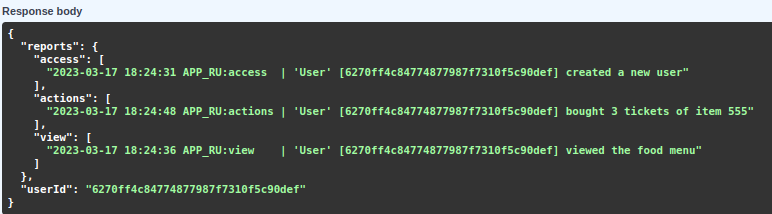
\includegraphics[width=1\textwidth]{img/Cap4/relatorio modulos.png}
    \caption{Visualização de histórico de interações de um usuário, separado por módulos}
    \label{fig:relatorio_modulos}
\end{figure}

\begin{figure}
    \centering
    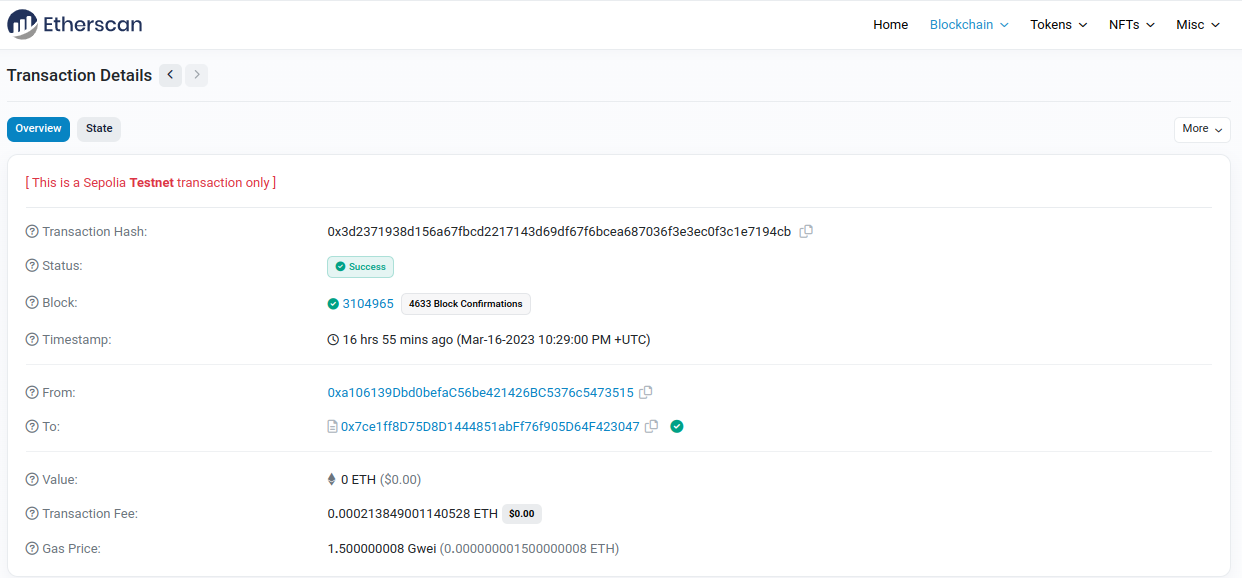
\includegraphics[width=1\textwidth]{img/Cap4/etherscan.png}
    \caption{Detalhes de uma transação via Etherscan}
    \label{fig:etherscan}
\end{figure}

Relatórios de uso do sistema podem ser gerados para usuários específicos por meio de sua identificação única. Existem dois \emph{endpoints} especiais na API que não geram mensagens de \emph{log}, um deles provê uma lista de todos as ações executadas por um usuário no sistema (Figura \ref{fig:trilha_auditoria}) enquanto que o outro lista as ações separadas por módulo. A separação das interações por módulo, conforme demonstrado na Figura \ref{fig:relatorio_modulos}, visa facilitar o processo de auditoria, listando as informações necessárias de acordo com o tipo de interação realizada pelo usuário. Desta forma, cada usuário possui um histórico próprio atrelado à Blockchain, sendo impossível ocorrer qualquer tipo de adulteração nos dados persistidos na rede.


\begin{figure}
    \centering
    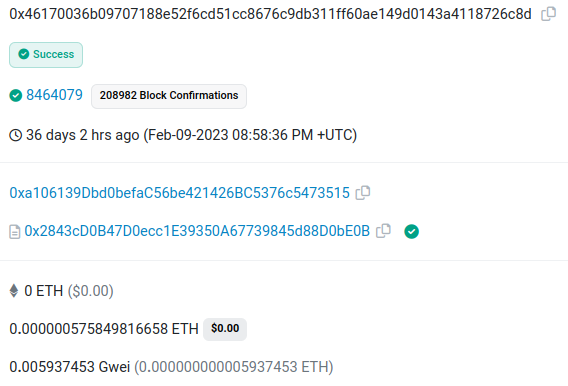
\includegraphics[width=0.45\textwidth]{img/Cap4/tx goerli.png}
    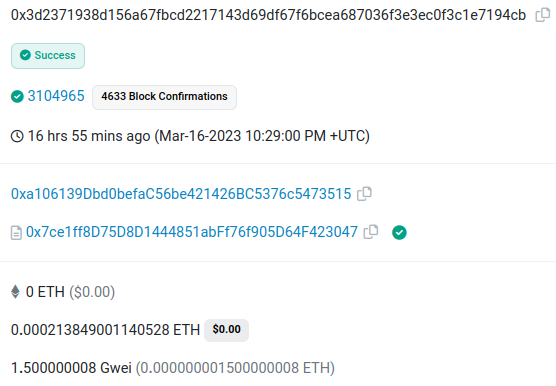
\includegraphics[width=0.45\textwidth]{img/Cap4/tx sepolia.png}
    \caption{Transações realizadas nas \emph{testnets} Goerli e Sepolia, respectivamente}
    \label{fig:preço_transacao}
\end{figure}

Todavia, observou-se que os custos operacionais relacionados a persistência mensagens de \emph{log} podem ser um aspecto impeditivo. Originalmente, a \emph{testnet} utilizada foi a rede Goerli, que possuía custos por transação viáveis; entretanto, durante o desenvolvimento deste trabalho a rede foi considerada como depreciada pelos desenvolvedores da Ethereum, ocasionando uma migração em massa para a rede Sepolia. Além disso, houveram variações no valor da criptomoeda Ether, a encarecendo. Com isto, o preço de \emph{gas} aumentou subitamente, tornando mais alto o preço das transações realizadas pelo sistema. A Figura \ref{fig:preço_transacao} demonstra a discrepância de valores entre as duas \emph{testnets}: supondo a cotação de 1 ETH como equivalente a R\$ 8.000,00, em fevereiro de 2023 o custo médio de uma transação realizada pela API REST custava em torno de R\$ 0,005 na rede Goerli; em março de 2023 uma transação variou de R\$ 1,00 a R\$ 2,50 na rede Sepolia. Isto impacta a viabilidade da solução. Porém, o sistema serviu o seu propósito como prova de conceito, e trabalhos futuros podem ser realizados para estudar métodos com o objetivo de aumentar a viabilidade da solução.

\section{Trabalhos futuros}
Como trabalhos futuros, melhorias ao sistema podem ser implementadas. Otimizações de custo operacional na Blockchain podem ser empregadas com o uso de formas mais sofisticadas de armazenamento de informações na rede, somado também a refatorações no contrato inteligente. Ethereum, por ser uma das redes Blockchain mais bem difundidas e utilizadas, possui taxas de \emph{gas} elevadas se comparada a outras redes Blockchain. Isto se deve a problemas de escalabilidade da plataforma, que pretendem ser sanados após a completa atualização da rede para a Ethereum 2.0. A rede Solana, por exemplo, possui um custo por transação de cerca de \$0.00025 USD por transação \cite{solana_compass}, ao passo que os valores rede Ethereum dependem do tráfego e do volume de transações da rede, podendo ser mais caros. Existem também alternativas livres de custo, como as criptomoedas NANO e TAMA \cite{analytics_insight}. Portanto, existe espaço para otimizar os custos envolvidos ao se executar uma transação na API REST desenvolvida.

Além disso, é possível otimizar o armazenamento de mensagens de \emph{log} salvas na rede. Ao invés de realizar a persistência diretamente no contrato inteligente, pode-se explorar diferentes maneiras de lidar com o fluxo de dados da aplicação. Uma alternativa é utilizar plataformas descentralizadas para armazenamento de arquivos, como o IPFS (InterPlanetary File System). Uma outra abordagem pode ser gerar valores \emph{hash} a partir da mensagem de \emph{log} criada e armazená-los na rede Blockchain, ao passo que a mensagem de \emph{log} em si junto com o \emph{hash} criado são armazenados em um banco de dados, de maneira local ou remota. Otimizar a persistência das mensagens de log é importante pois métodos alternativos têm a possibilidade de serem bem menos dispendiosos em termos de valor de transação e preço de \emph{gas}.

Outro fator importante a ser levado em consideração é a quantidade de informações que são persistidas na rede. O sistema desenvolvido salva toda e qualquer interação realizada pelo usuário dentro do contexto do aplicativo da Carteira Digital do Restaurante Universitário da UEA. É interessante realizar um levantamento acerca de quais são as informações essenciais para serem salvas na rede a fim de que se possa haver processos de auditoria. Dados como registrar que o usuário visualizou a seção de comentários ou o cardápio, por exemplo, podem não ser tão valiosos quando se comparado ao registro de ações-chave no sistema, como a compra de um ticket.



% Referência segundo o padrão ABNT
% Edite este arquivo e inclua suas referências segundo a notação do Bibtex
\bibliography{ref}



\end{document}
